\documentclass[12pt,a4paper]{report}
\usepackage[utf8]{inputenc}
\usepackage{graphicx}
\graphicspath{ {C:/Users/kamila/Documents/Praca licencjacka/} }
\usepackage{amsmath}
\usepackage{tikz}
\usepackage{amsfonts}
\usepackage{latexsym}
\usepackage{amssymb}
\usepackage{amsthm}
\usepackage{paralist}
\usepackage{polski}
\usepackage{xcolor}
\usepackage{multicol}
\usepackage[hidelinks]{hyperref}
\usepackage{natbib} % potrzba do bibliografii
\usepackage[left=2cm,right=2cm,top=2cm,bottom=2cm]{geometry}
%\usepackage[acronym]{glossaries} COS NIE DZIALA WYWALA BLEDY

\author{Kamila Choja}
\title{Wybrane zastosowanie statystycznych metod porządkowania danych wielowymiarowych}


\newtheorem{theorem}{Twierdzenie}[section]
\newtheorem{definition}[theorem]{Definicja}
\newtheorem{uwaga}{Uwaga}
\newtheorem{example}{Przykład}
\newtheorem{stwierdzenie}{Stwierdzenie}
\newtheorem{wlasnosci}{Własności}

\newcommand{\setR}{\mathbb{R}}

\newcommand{\Lp}[2]{\operatorname{L}_{#1} \left( {#2} \right)}
\newcommand{\norm}[2][]{\left\| {#2} \right\|_{#1}}
\newcommand{\distance}[3][d]{\operatorname{#1}\left( {#2}; {#3}\right)}
\newcommand{\mediana}{\operatorname{med}}
\newcommand{\licznosc}[1]{\overline{\overline{#1}}}

\newcommand{\Ex}{\operatorname{E}}
\newcommand{\Variance}{\operatorname{Var}}

\newcommand{\closure}[1]{\overline{#1}}

\begin{document}
\begin{titlepage}
\begin{center}
        \vspace*{1cm}
        {\large POLITECHNIKA ŁÓDZKA}\\
       \vspace*{1cm}
        {\large WYDZIAŁ FIZYKI TECHNICZNEJ, INFORMATYKI I MATEMATYKI STOSOWANEJ}\\
        \vspace*{2cm}
    \end{center}        
        
\text{Kierunek: Matematyka}\\
\vspace*{0.3cm}
\hspace*{0.3cm}
\text{Specjalność: Matematyczne Metody Analizy Danych Biznesowych}
  
\begin{center}
\rule{\textwidth}{0.5pt}

\vspace*{0.5cm}
   
{\large WYBRANE ZASTOSOWANIE STATYSTYCZNYCH METOD\\ }
{\large PORZĄDKOWANIA DANYCH WIELOWYMIAROWYCH\\}
\vspace*{1cm}


\begin{flushright}
Kamila Choja\\
Nr albumu: 204052 
 \end{flushright}
\rule{\textwidth}{0.5pt}

Praca licencjacka\\
napisana w Instytucie Matematyki Politechniki Łódzkiej\\

\vspace*{2cm}

Promotor: dr, mgr inż. Piotr Kowalski\\
\vfill
ŁÓDŹ, xxx 2018


     \end{center}   
\end{titlepage}

\tableofcontents

\chapter{Wstęp}
Wielowymiarowa analiza danych jest pojęciem dosyć nowym, jedną z jej części są metody porządkowania. Aby móc w pełni zrozumieć to zagadnienie, należy przyjrzeć się podłożu matematycznemu tego tematu. 
Dane które chcemy poddać analizie, są niczym innym jak próbą losową, składającą są z niezależnych zmiennych losowych, w związku z tym w sekcji \ref{rachunek prawdopodobienstwa} zostały przytoczone podstawowe pojęcia rachunku prawdopodobieństwa oraz statystyki, dzięki temu w dalszej części pracy łatwiej zrozumieć zbiór danych jako zbiór obiektów, opisywanych przez zmienne. Mając opracowane te zagadnienia, mogłam przejść do matematycznej interpretacji porządku, gdyż czym tak naprawdę on jest? Otóż porządek to nic innego jak relacja porządku, który możemy podzielić na porządek liniowy - czyli tę relację która umożliwia nam porównywanie każdych dwóch obiektów między sobą, a także na porządek częściowy który to podobnie jak relacja porządku liniowego umożliwia porównywanie obiektów między sobą, aczkolwiek nie zachodzi to na wszystkich elementach danego zbioru, zatem nie jest spełniony warunek spójności. Ze względu na powyższe została opracowana sekcja \ref{teoria mnogosci}, w której umieściłam wszystkie niezbędne definicje z zakresu teorii mnogości z których korzystam w pracy. 

W dalszej części pracy zostały opracowane podstawowe pojęcia teorii grafów \ref{grafy}, spowodowane to zostało interpretację graficzną częściowego uporządkowania zbioru, którego to metody statystyczne opracowane na podstawie \citep{panek2013} zostały przedstawione obok metod porządkowania liniowego w rozdziale \ref{metody porzadkowania}. Ze względu na to również, że część praktyczna pracy, została w większości oparta na podstawie  tej pozycji, użyłam przyjętych przez autora nazw statystycznych podziału relacji porządku, tj. metody porządkowania liniowego, natomiast metody będące odpowiednikiem relacji częściowego porządku zostały umieszczone pod nazwą metody porządkowania nieliniowego. Pozostając przy rozdziale \ref{metody porzadkowania} na samym jego początku zostały omówione własności porządkowania liniowego, które to w dalszej  kolejności zostały sformalizowane, a następnie udowodnione. 
Ostatni rozdział pracy \ref{Zastosowanie} stanowi jej praktyczny aspekt. Omówiłam w nim stworzony przez siebie zbiór danych, na którym to w dalszej części pracy przetestowałam stworzone przez siebie implementacje wybranych metod porządkowania. Algorytmy zostały napisane w programie R-Studio.  Na koniec wyniki uporządkowań zostały porównane.

%Przy metodach porządkowania warto wspomnieć o interpretacji geometrycznej uporządkowania. W przypadku relacji częściowego porządku, interpretacją jest diagram Hassego, w którym to dany obiekt łączy jest z drugim, gdy jeden jest poprzednikiem drugiego, a drugi jest następnikiem pierwszego. %%odwolanie do sekcji grafy slabe - pomyslec; moze niezbendym bylo opracowanie podstawowoych pojec z teorii grafow, ze wzgledu na to ze w roddziale 3 - odwolanie, opracowanym na podstawie ksiazki \cite{panek2013} zostały tam omówione statystyczne metody porządkowania - liniowe i nieliniowe. Powracajac do ujecie matemtycznego, te drugie sa niczym innym jak interpretacja relacji czesciowego porzadku
%Jako że w dalszej części pracy zostały przedstawione 
%%pomyslec odowloanie do grafu i metod prozadkowania w jendym
%Po wprowadzeniu powyższych pojęć, mogłam przejść do części praktycznej pracy tj. implementacji wybranych %zastosowań metod porządkowania. W związku z tym został stworzony rozdział 4 \ref{Zastosowanie}, w którym to %omówiłam stworzony przez siebie zbiór obiektów, a następnie zaprezentowałam własne algorytmy wybranych metod, które zostały opracowane z wykorzystaniem R-Studio.




% W ujęciu matematycznym porządkowanie jest niczym innym jak relacją porządku, który możemy podzielić na porządek liniowy oraz częściowy na danym zbiorze. Ze względu na to, w sekcji \ref{teoria mnogosci} zostały opracowane wybrane pojęcia teorii mnogości, po to by w dalszej części pracy móc przejść do  Niezbędnym również było wprowadzenie podstawowych pojęć rachunku prawdopodobieństwa, w celu zrozumienia danych jako próby losowej, w tym celu została stworzona sekcja \ref{rachunek prawdopodobienstwa}. Mając tak opracowane podstawy teoretyczne mogłam przejść do 

%W rozdziale 3 zostaną omówione implementacje porządku liniowego jak i częściowego. Ze względu na to, że część praktyczna pracy, została w większości oparta na książce \cite{panek2013}, w związku z tym użyłam przyjętych przez autora nazw statystycznych podziału relacji porządku, tj. metody porządkowania liniowego, natomiast metody będące odpowiednikiem relacji częściowego porządku zostały umieszczone pod nazwą metody porządkowania nieliniowego. 

\chapter{Preliminaria}  

\section{Notacja} 

Poniżej znajduje się lista pojęć powszechnie używanych w pracy wraz z symbolami, które im się przypisuje. 
  
\begin{itemize}
\item $\mathbb{R}$ - zbiór liczb rzeczywistych
\item $\mathbb{N}$ - zbiór liczb naturalnych
%\item $\licznosc{[1]}$ - liczność zbioru
%+-\item $\mathcal{E}^n$ - przestrzeń euklidesowa n-wymiarowa
\item O = $\{$O$_{1}$, O$_{2}$, $\dots$, O$_{n}\}$ - zbiór obiektów przestrzennych, tj. opisywanych przez wiele atrybutów, $n \in \mathbb{N}$
\item $X=[x_{ij}]$ - macierz danych, gdzie $x_{ij}$-oznacza wartość $j$-tej zmiennej dla $i$-tego obiektu, gdzie $i=1,\ldots,n$, $j=1,\ldots, m,$, $n,m \in \mathbb{N}$
\item $n_{ij}$ -oznaczenie znormalizowanej wartości $j$-tej cechy $i$-tego obiektu
\item $x^{S}$ - oznaczenie zmiennej mającej charakter stymulanty
\item $x^{D}$ - oznaczenie zmiennej mającej charakter destymulanty
\item $x^{N}$ - oznaczenie zmiennej mającej charakter nominanty
\item $D=[d_{ik}]$ - oznaczenie macierzy odległości, gdzie $d_{ik}$ oznacza odległość między $i$-tym i $k$-tym obiektem
\item $s_{i}$ - oznaczenie zmiennej syntetycznej $i$-tego obiektu
\item $P_{0}=[n_{0j}]$ - oznaczenie obiektu wzorcowego, gdzie $n_{0j}$- znormalizowana $j$-ta współrzędna obiektu wzorcowego
\item $X$ - w rozdziale drugim przez $X$ najczęściej oznaczać będziemy dowolny zbiór, jednak w dalszych rozdziałach najczęściej służyć on będzie do opisywania macierzy zawierającej podstawowe (surowe) dane do analizy
\item $Y$ - w rozdziale drugim używana jest najczęściej do oznaczenie zmiennej losowej
\item $\Omega$ - oznaczenie dowolnej przestrzeni zdarzeń elementarnych $\omega$, z rodziną podzbiorów $\mathcal{F}$
%\item $\sigma$ -  sigma ciało zbiorów $\mathcal{F}$
\item $\mathcal{B}$ - rodzina zbiorów borelowskich
\item $\mathfrak{B}$ - rodzina wszystkich zbiorów otwartych %https://www.sharelatex.com/learn/Mathematical_fonts
%\item $\mediana ( \cdot)$ - oznaczać będzie mediany z próby
\item $\leq$ - oznaczenie relacji częściowego porządku, przy dołożeniu warunku spójności oznaczać będzie relację liniowego porządku
\item $G$ - oznaczenie ogólnego grafu prostego dla którego $V(G)$ jest zbiorem wierzchołków grafu, a $E(G)$ zbiorem jego krawędzi


%\item $D$ - graf skierowany(digraf)
%\item $V(D)$ - zbiór wierzchołków digrafu $D$
%\item $A(D)$ - rodzina łuków digrafu $D$


\end{itemize}


\section{Słownik użytych pojęć}
W pracy zostały wykorzystane następujące pojęcia, których wytłumaczenie znajduje się poniżej. 
\begin{itemize}
%pojecia proby,statystyi, modelu - formalne mozna podac w oparciu o wyklady Bartoszewicza i pliku- "proba_mod staty_statytsyka folder: pliki pdf do pracy
\item Statystyka matematyczna \cite[w oparciu o rozdział 1]{krysicki1999}
Statystyka matematyczna zajmuje się opisywaniem i analizą zjawisk przy użyciu metod rachunku prawdopodobieństwa. 


%\item Model statystyczny \cite[w oparciu o rozdział 2]{bartoszewicz1996}
%Modelem statystycznym nazywamy przestrzeń próby doświadczenia tj. wartości zmiennych losowych o jednakowym rozkładzie, rodzinę podzbiorów zbioru zmiennych oraz prawdopodobieństwo występowania danej zmiennej. Można tutaj wskazać analogię do rachunku prawdopodobieństwa, tj. uporządkowanej trójki $(\Omega,\mathcal{F},P)$.
 
 
\item Cecha statystyczna \cite[Rozdział 1]{krysicki1999}
Cecha statystyczna jest to właściwość wspólna dla danego zbioru obserwacji. Jej wartości pozwalają rozróżnić elementy zbioru między sobą. cechy statystyczne można podzielić na te mierzalne, tj. ilościowe (np. długość, ciężar), oraz niemierzalne tj. jakościowe(np. kolor, płeć, zawód, województwo).

\end{itemize}

W celu prezentacji dużych ilości danych, w analizie danych korzysta się z pojęcia macierzy. Poniżej zostanie przedstawiona definicja macierzy obserwacji, czyli zbiorowi obiektów, opisywanych przez zmienne. W rozdziale dotyczącym Wybranych pojęć z teorii mnogości, topologii oraz algebry liniowej, zostanie podana jej algebraiczna definicja. 


\begin{definition}[{Macierz obserwacji \cite[Rozdział 2]{mlodak2006}}]
Niech $m>1$ oraz $n>1$ będą liczbami naturalnymi.  Macierzą obserwacji nazywamy macierz rozmiaru  $n \times m$  postaci
$$
X= \begin{bmatrix}
x_{11} & x_{12} & \ldots & x_{1m} \\
x_{21} & x_{22} & \ldots & x_{2m}\\
\ldots & \ldots & \ldots & \ldots \\
x_{n1} & x_{n2} & \ldots & x_{nm}\\
\end{bmatrix}
$$
gdzie:
* $x_{ij}$ - zaobserwowana wartość $j$-tej cechy dla $i$-tego obiektu .
\end{definition}


\begin{definition}{Macierz odległości zmiennych \cite[Rozdział 1.6]{panek2013}}
Macierzą odległości cech zmiennych nazywamy macierz, której elementami są odległości między parami badanych obiektów: 
\begin{center}
$D = [d_{ik}].$\\
\end{center}
gdzie:\\
$dik$-odległość między $i$-tym a $k$-tym obiektem, dla $i,k=1,2,\ldots,n$
\end{definition}

W statystyce posługujemy się pojęciami skal do opisu różnych typów danych, które mogą podlegać naszej analizie. I tak zdefiniujmy następujące rodzaje skal:

\begin{itemize}
%poprawic
\item Skala \cite[w oparciu o rozdział 1.2]{panek2013}
Skalą nazywamy pewien skończony zbiór, umożliwiający porównywanie obiektów na podstawie wartości lub własności wybranych zmiennych.

\item Skala porządkowa \cite[Rozdział 1.2]{panek2013}
Skala ta umożliwia sprawdzenie identyczności, różnicy obiektów które są porównywane. Pozwala również na porównaniu wariantów cech, które opisują obiekty. Za jej pomocą nie można jednak na określić odległości między obiektami. Umożliwia zliczanie uporządkowanych obiektów (liczby relacji równości, nierówności, większości i mniejszości). Przykład zmiennych przedstawianych na skali porządkowej: wykształcenie, kolejność zawodników na podium, oceny w systemie szkolnym.

\item Skala przedziałowa \cite[Rozdział 1.2]{panek2013}
Jest to skala, która w odróżnieniu do skali porządkowej, pozwala obliczyć odległość między obiektami, przy pomocy pomiaru cech, opisujących obiekt. Skala ta może korzystać z operacji dodawania oraz odejmowania. Dla skali tej istnieje charakterystyczna wartość - punkt zerowy. Jest on wyznaczany w sposób umowny, punkt ten pozwala zachować różnice między wartościami cechy, w momencie zamiany jednostek miary. Przykład zmiennych przedstawianych na skali przedziałowej: temperatura, rok urodzenia. %Wartość zerowa na tej skali ma charakter umowny, co prowadzi do zachowania różnic między wartościami cechy, przy zmianie jednostek miary. 

\item Skala ilorazowa \cite[Rozdział 1.2]{panek2013}
Skala ta, podobna jest do skali przedziałowej, z tym że występuje w niej zero bezwględne - punkt, który mówi o tym, że dana zmienna nie występuje, oraz ogranicza lewostronnie zakres skali ilorazowej. Dzięki temu punktowi oprócz działań dodawania i odejmowania, można korzystać z dzielenia oraz mnożenia, co pozwala na przedstawieniu dowolnej wartości cechy danego obiektu, jako wielokrotna wartość cechy innego obiektu. Przykład zmiennych przedstawianych na skali ilorazowej: napięcie elektryczne, bezrobocie, inflacja.

%\item Zmienna objaśniająca \cite[Rozdział 1.1] {grabinski1982}
%Zmienną objaśniającą nazywamy zmienną w modelu statystycznym, która oddziałuje na zmienne objaśniane. Zmiennie  %objaśniającą oznaczamy jako $X_{1}, ldots, X_{k}$, z kolei zmienne objaśniane jako $Y$. \\
\end{itemize}

\begin{definition}{Stymulanta \cite[Rozdział 1.5]{panek2013}}
Stymulantami nazywane są zmienne(cechy), dla których pożądane są wysokie wysokie wartości w badanych obiektach, ze względu na rozpatrywane zjawisko. 
\end{definition}

\begin{definition}{Destymulanta \cite[Rozdział 1.5]{panek2013}}
Destymulantami nazywane są zmienne, dla których niepożądane są wysokie wysokie wartości w badanych obiektach, ze względu na rozpatrywane zjawisko. 
\end{definition}

\begin{definition}{Nominanta \cite[Rozdział 1.5]{panek2013}}
Nominantami nazywane są zmienne, które mają z góry określoną najkorzystniejszą wartość. Odchylenia od tej wartości są niepożądane, ze względu na rozpatrywane zjawisko. 
\end{definition}



%\item Stopień podobieństwa obiektów \cite[Rozdział 1.6]{panek2013}\\
%Stopień podobieństwa obiektów, jest wielkość mówiąca o podobieństwie obiektów między sobą. Jest on mierzony za pomocą miar odległości lub tez miar bliskości(zgodności).\\

%\item Miara odległości \cite[Rozdział 1.6]{panek2013}\\
%Miarą odległości pomiędzy obiektami: $i$-tym i $k$-tym, nazywamy dowolną funkcję rzeczywista $d$, spełniającą następujące %warunki:\\
%- {\bf dodatniość} (odległość między różnymi obiektami jest zawsze dodatnia): $d_{ik}>0$\\
%- {\bf symetryczność} (odległość $i$-tego obiektu od $k$-tego obiektu jest taka sama, jak odległość $k$-tego obiektu od 		obiektu $i$-tego: $d_{ik}=d_{ki}$\\
%- {\bf zwrotność} (odległość obiektu od samego siebie jest równa zeru): $d_{ii}=0$\\
%- {\bf nierówność trójkąta}: odległość pomiędzy $i$-tym i $k$-tym obiektem będzie nie większa niż odległość pośrednia pomiędzy tymi obiektami definiowana jako suma odległości pomiędzy obiektami $i$-tym i $k'$-tym oraz $k$-tym i $k'$-tym): $d_{ik} \leq d_{ik'} + d_{k'k}$.\\

%\begin{uwaga}
%Wzrost wartości miary odległości oznacza zmniejszenie stopnia podobieństwa obiektów.\\
%\end{uwaga}

%\item Odległość euklidesowa dla znormalizowanych zmiennych \cite[Rozdział 1.6]{panek2013}\\
%Wzór odległości euklidesowej, dla znormalizowanych zmiennych, jest następujący:
%\begin{center}
%$$d_{ik}=\big[\sum_{j=1}^{m}|z_{ij}-z_{kj}|^{2} \big]^{\frac{1}{2}}$$
%\end{center}

%\item Odległość miejska(Manhattan) dla znormalizowanych zmiennych \cite[Rozdział 1.6]{panek2013}\\
%Wzór na odległość miejską(Manhattan) dla znormalizowanych zmiennych, jest następujący:
%\begin{center}
%$$d_{ik}=\sum_{j=1}^{m}|z_{ij}-z_{kj}|.$$
%\end{center}

%\item Miara bliskości \cite[Rozdział 1.6]{panek2013}\\
%Miarą bliskości pomiędzy obiektami, nazywamy funkcję $p$ spełniającą następujące warunki:\\
%- {\bf dodatniość}: $p_{ik} > 0$,\\
%- {\bf symetryczność}: $p_{ik} = p_{ki}$\\
%- {\bf zwrotność}: $p_{ii} = 1$.\\
%: Wzrost wartości miary bliskości oznacza zwiększenie stopnia podobieństwa badanych obiektów.\\

%\item Macierz odległości \cite[Rozdział 1.6]{panek2013}\\
%Macierzą odległości, nazywamy macierz unormowanych danych wejściowych, tj. macierz, której elementami są odległości między %parami badanych obiektów. Macierz odległości jest postaci:
%\begin{center}
%$D = [d_{ik}], i,k=1, 2, ..., n.$\\
%\end{center}

%\item Średnia arytmetyczna z próby \cite[Rozdział 2.2]{mlodak2006}\\
%Średnią arytmetyczną wartości cechy $X_{j}$ nazywamy wartość 
%\begin{center}
%$$\overline{x_{j}}= \frac{\sum_{i=1}^{n} x_{ij}}{n}$$\\
%\end{center}

%\item Odchylenie standardowe z próby \cite[Rozdział 2.2]{mlodak2006}\\
%Odchyleniem standardowym cechy $X_{j}$  nazywamy wartość 
%\begin{center}

%$$s_{j}= \sqrt{ s_{j}^2} = \sqrt{\frac{1}{n}\sum_{i=1}^{n} (x_{ij} - \overline{x_{j}})^2}$$\\

%\end{center}

%\item Mediana \cite[Rozdział 2.2]{mlodak2006}\\
%Medianę cechy $X_{j}$ nazywamy wartość \\
%\begin{center}

%med$(X_{j})= 
%y = \left\{ \begin{array}{ll}
%\frac{1}{2}\big(x_{(\frac{n}{2})j} + x_{(\frac{n}{2}+1)j}\big) & \textrm{jeśli n jest parzyste} \\\\
%x_{(\frac{n+1}{2})j} & \textrm{jeśli n jest nieparzyste}\\

%\end{array} \right.
%$\\
%\end{center}

%\item Przestrzeń euklidesowa n-wymiarowa $\mathcal{E}^n$ \citep[Rozdział 9]{kuratowski2004}\\
%Przestrzeń euklidesowa n-wymiarowa, jest przestrzenią metryczną przy zwykłej definicji odległości punktu %$x=(x_1,x_2,...,x_n)$ od punktu $y=(y_1,y_2,...,y_n)$, danej wzorem Pitagorasa
%\begin{center}
%$$|x - y| =\sqrt{\sum_{i=1}^{n} |x_i - y_i|^2}$$
%\end{center}
%gdzie, $x$ i $y$ są ciągami złożonymi z n liczb rzeczywistych.

%\item Obiekt wzorcowy \cite[Rozdział 2.2]{panek2013}\\
%Obiektem wzorcowym nazywany jest obiekt modelowy o pożądanych wartościach zmiennych wejściowych.\\

%\item Obiekt wzorcowy \cite[Rozdział 2.1]{mlodak2006}\\
%Obiektem wzorcowym, nazywamy obiekt powstały na podstawie macierzy wystandaryzowanych zmiennych wejściowych. Współrzędnymi obiektu są: \\
%\begin{center}

%$O_{0}=[z_{0j}], j= 1,2,...,m.$\\

%\end{center}
%gdzie współrzędne obiektu wzorcowego obliczane są na podstawie wzoru:
%\begin{center}
%$z_{oj}=max_{i}$
%\end{center}
%\begin{equation}
%z_{oj}=\left\{ \begin{array}{ll}
%\max\limits_{i} \Big\{z_{ij}\Big\}  & \textrm{dla  } z_{j}^S\\\\
%\min\limits_{i}\Big\{ z_{ij} \Big\} & \textrm{dla } z_{j}^D\\
%\end{array} \right.
%\end{equation}
%gdzie:
%\\*$j=1,2,...,m; i=1,2,...,n.$\\


%\item Funkcja kryterium dobroci uporządkowania \cite[Rozdział 2.2]{panek2013}\\
%Funkcją kryterium dobroci uporządkowania nazywamy funkcję: 
%\begin{center}
%$$F^2= \sum_{k=1}^{n-1} k \sum_{i=1}^{n-k} d_{ik}$$\\

%\end{center}
%gdzie:
%\\* $d_{i,k}$ - odległość euklidesowa między $i$-tym i $k$-tym obiektem . \\



%\begin{definition}{Współczynnik Pearsona \cite[Rozdział 2.2]{mlodak2006}\\}
%Współczynnik Pearsona oznaczamy: 
%\begin{center}
%$r_{jk}= \frac{\mathrm{cov}(X_{j},X_{k})}{s_{j}s_{k}}$\\

%\end{center}
%gdzie:
%\\* $\mathrm{cov}(X_{j},X_{k})$ - kowariancja cech $X_{j}$ i $X_{k}$ .\\
%\end{definition}

\

\subsection{Wybrane operacje statystyczne dla zmiennych}
\subsubsection{Normalizacja zmiennych}
Bardzo ważnym krokiem przed rozpoczęciem pracy na zbiorze danych jest ujednolicenie ich charakteru, tj. przekształcenie zmiennych (mierzonych na skali przedziałowej lub ilorazowej) opisujących obiekty w zbiorze, w celu pozbycia się dysproporcji między nimi czy też dominacji jednych zmiennych nad drugimi. W tym celu stosuje się transformację normalizacyjną. Można wyróżnić trzy podstawowe typy przekształceń normalizacyjnych:
\begin{itemize}
\item standaryzacja,
\item unitaryzacja,
\item przekształcenie ilorazowe
\item rangowanie zmiennych
\end{itemize}
W dalszej części pracy $j$-ta zmienna znormalizowana, $i$-tego obiektu jest oznaczona jako $n_{ij}$.
\begin{enumerate}
\item W wyniku standaryzacji zmienne uzyskują odchylenie standardowe równe 1 i wartości oczekiwanej  równą 0. W tym celu dla każdej zmiennej, będącej cechą obiektu oblicza się odchylenie standardowe na podstawie wartości tej zmiennej dla wszystkich obiektów, a także wartość oczekiwaną na tej samej zasadzie. W kolejnym kroku dla każdego obiektu liczymy jego znormalizowana wartość tj. od wartości zmiennej odejmujemy wartość oczekiwaną dla danej cechy, a otrzymaną różnicę dzielimy przez odchylenie standardowe dla tej cechy,co można to zapisać w postaci
$$
n_{ij}=\frac{x_{ij} - \Ex (x_j)}{\sigma(x_j)}, \quad i = 1,2, \ldots, n, \quad j=1,2,\ldots, m.
$$
gdzie
$z_{ij}$-wartość znormalizowanej zmiennej $j$-tej zmiennej, w $i$-tym obiekcie.


\item W pracy skorzystałam również z unitaryzacji, stosowanej w celu uzyskania zmiennych o ujednoliconym zakresie zmienności, u mnie przedział ten to $[0,1]$. W tym celu od wartości zmiennej w obiekcie, odejmowana jest minimalna wartość występująca dla tej cechy, a następnie różnica ta dzielona jest przez różnicę między maksymalną a minimalną wartością zmiennej, która została poddana normalizacji. Znormalizowana zmienna jest postaci
$$
n_{ij}=\frac{x_{ij} - \min\limits_{i}\{x_{ij}\}}{\max\limits_{i} \{x_{ij}\} - \min\limits_{i} \{x_{ij}\}}, \quad i = 1,2, \ldots, n, \quad j=1,2,\ldots, m. 
$$
\item Kolejna metoda normalizacyjna, wykorzystana w pracy to przekształcenie ilorazowe. Stosuje się  je aby odnieść wartości zmiennej do ustalonej wartości - może to być wartość oczekiwana danej zmiennej na tle analizowanych obiektów, wartość minimalna lub maksymalna tej cechy. W pracy za tę wartość przyjęłam wartość oczekiwaną zmiennej. Każda wartość zmiennej dla danego obiektu jest dzielona przez wartość oczekiwaną tej zmiennej, a postać znormalizowanej zmiennej to
$$
n_{ij}=\frac{x_{ij}}{\Ex (x_j)}, \quad \Ex (x_j) \neq 0 \quad i = 1,2, \ldots, n, \quad j=1,2,\ldots, m.
$$ 
\item Przy zastosowaniu metody rang, wykorzystuje się normalizację rangową. Przekształcenie to, najczęściej stosowane jest, gdy zmienne opisujące obiekty są wyrażone na skali porządkowej. W pierwszym kroku wartości zmiennych opisujących obiekty zostają uporządkowane ze względu na ich wartości po procesie normalizacji. W kolejnym kroku wartościom zmiennej przyporządkowywane są rangi - czyli wartości liczbowe, będące najczęściej numerami miejsc zajmowanych przez obiekty w uporządkowanym zbiorze. Postać zmiennej znormalizowanej rangowo
$$
n_{ij}=r, \quad dla x_{hj}=x_{ij}, \quad i = 1,2, \ldots, n, \quad j=1,2,\ldots, m.
$$
gdzie 
$r$-ranga nadana $i$-temu obiektowi znajdującemu się na $r$-tym miejscu w uporządkowanym zbiorze, ze względu na wartość $j$-tej zmiennej. 
\end{enumerate}

\subsubsection{Stymulacja zmiennych}
W celu ujednolicenia charakteru danych należy poddać je pewnym przekształceniom, polegającym na zamianie destymulant i nominant na stymulanty. Tego typu transformacje nazywamy stymulacją. Można wyróżnić dwie najczęściej stosowane metody, tj. przekształcenie ilorazowe oraz przekształcenie różnicowe. W zależności od skali na której mierzone są zmienne, należy stosować odpowiednie przekształcenie stymulacyjne.

W przypadku przekształcenia ilorazowego można go stosować tylko dla zmiennych mierzonych na skali ilorazowej. Stymulacja destymulant wygląda następująco
$$
x_{ij}^{S}=[x_{ij}^{D}]^{-1},  \quad i = 1,2, \ldots, n, \quad j=1,2,\ldots, m.
$$
dla nominant
$$
x_{ij}^{S}=\frac{\max\{x_{j}^{N},x_{ij}^{N}\}}{\max\{x_{j}^{N},x_{ij}^{N}\}}, \quad i = 1,2, \ldots, n, \quad j=1,2,\ldots, m.
$$

Dla zmiennych mierzonych na skali ilorazowej czy też przedziałowej stosuje się przekształcenie różnicowe. Stymulacja dla destymulant prezentuje się następująco
$$
x_{ij}^{S}=\max\limits_{i} \{x_{ij}^{D}\} - x_{ij}^{D}, \quad i = 1,2, \ldots, n, \quad j=1,2,\ldots, m,
$$
a dla nominant
$$
x_{ij}^{S}=-|x_{ij}^{N}-x_{j}^{N}|, \quad i = 1,2, \ldots, n, \quad j=1,2,\ldots, m.
$$





\section{Podstawowe pojęcia rachunku prawdopodobieństwa oraz statystyki} \label{rachunek prawdopodobienstwa}


Na potrzeby pracy, zostały wykorzystane pojęcia rachunku prawdopodobieństwa oraz statystyki, konieczne do zrozumienia danych jako próby losowej. W tym celu niezbędne było wprowadzenie definicji prawdopodobieństwa, zmiennej losowej, a także pojęć powiązanych z tymi definicjami tj. ciała zbiorów, $\sigma$-ciała zbiorów, przestrzeni zdarzeń elementarnych, zdarzenia losowego.


\begin{definition}{Ciało zbiorów \cite[Rozdział 8.1]{rudnicki2006}}
Rodzinę $\mathcal{F}$ podzbiorów, niepustego zbioru $Y$ nazywamy ciałem zbiorów, jeżeli spełnia ona następujące warunku: 
\begin{enumerate}
\item $\emptyset \in \mathcal{F}$,
\item jeżeli $A \in \mathcal{F}$, to $Y \setminus A \in \mathcal{F}$,
\item jeżeli $A \in \mathcal{F}$, to $A \cup B \in \mathcal{F}$.
\end{enumerate}
\end{definition}


\begin{definition}{$\sigma$-algebra/ciało zbiorów\cite[Rozdział 8.1]{rudnicki2006}}
Ciało zbiorów $\mathcal{F}$ nazywamy $\sigma$-ciałem zbiorów, jeżeli spełnia ona warunek
dla dowolnych zbiorów $A_{n} \in \mathcal{F}, n \in \mathbb{N}$, mamy
$\bigcup\limits_{i=1}^{\infty} A_n \in \mathcal{F}$.

%Elementy $\sigma$-ciała $\mathcal{F}$ nazywamy zbiorami mierzalnymi.
\end{definition}


\begin{definition}{Zbiory borelowskie \cite[w opraciu o rozdział 2]{billingsley1987}}
Zbiorami borelowskimi względem danej przestrzeni $Y$, nazywamy zbiory należące do $\sigma$-ciała $Y$ generowanego przez rodzinę $\mathfrak{B}(Y)$ - wszystkich zbiorów otwartych w $Y$. Rodzinę wszystkich zbiorów borelowskich względem $Y$, oznaczamy $\mathcal{B}(Y)$.
\end{definition}


\begin{definition}{Przestrzeń zdarzeń elementarnych \cite[w oparciu o rozdział 1.1]{krysicki1999}}
Zbiór wszyskich możliwych wyników doświadczenia losowego nazywamy przestrzenią zdarzeń elementarnych i oznaczamy przez $\Omega$. Elementy zbioru $\Omega$ nazywamy zdarzeniami elementarnymi i oznaczamy $\omega$.
\end{definition}


\begin{definition}{Miara zbioru \cite[Rozdział 2.10] {billingsley1987}}
Funkcję $\mu$ określoną na ciele $\mathcal{F}$ podzbiorów zbioru $\Omega$ nazywamy miarą, jeśli spełnia następujące warunki: 
\begin{enumerate}
\item $\mu(A) \in [0, \infty]$ dla każdego zbioru $A \in \mathcal{F}$,
\item $\mu(\emptyset)=0$,
\item jeśli $A_1, A_2,...$ jest ciągiem rozłącznych zbiorów $\mathcal{F}$-mierzalnych takich, że $\bigcup\limits_{k=1}^{\infty} A_k \in \mathcal{F}$, to 

$$\mu\big(\bigcup\limits_{k=1}^{\infty} A_k\big)=\sum_{k=1}^{\infty} \mu(A_k)$$

\end{enumerate}
\end{definition}


\begin{definition}{Przestrzeń mierzalna \cite[Rozdział 2.10]{billingsley1987}}
Przestrzenią mierzalną nazywamy parę $(Y, \mathcal{F})$, gdzie $\mathcal{F}$ jest $\sigma$-ciałem podzbiorów zbioru $Y$
\end{definition}


\begin{definition}{Funkcja mierzalna \cite[w oparciu o rozdział 8.2]{rudnicki2006}}
Niech $Y$ będzie niepustym zbiorem, $\mathcal{F}$  $\sigma$-ciałem na $Y$ i $\overline{\mathbb{R}} = \mathbb{R} \cup \{-\infty, \infty \}$. Funkcję $f: Y \rightarrow \overline{\mathbb{R}}$ nazywamy mierzalną, jeżeli zbiór
$\{ y \in Y: f(y) > a \}$

jest mierzalny przy dowolnym $a \in \mathbb{R}$.
\end{definition}


\begin{definition}{Zdarzenie losowe \cite[w oparciu o rozdział 1.1]{krysicki1999}}
Zdarzeniem losowym (zdarzeniem) nazywamy każdy podzbiór $\textit{A}$ zbioru $\Omega$, taki że  $A \in \mathcal{F}$, gdzie $\mathcal{F}$ jest rodziną podzbiorów $\Omega$ spełniającą następujące warunki:
\begin{enumerate}
\item $\Omega \in \mathcal{F}$;
\item Jeśli $A \in \mathcal{F}$, to $\textit{A$'$} \in \mathcal{F}$, gdzie $\textit{A$'$} = \Omega \setminus A $ jest zdarzeniem przeciwnym do zdarzenia $\textit{A}$;
\item Jeśli $\textit{A}_{i} \in \mathcal{F}$, $i= 1, 2, ...$,to $\bigcup\limits_{i=1}^{\infty} A_{i} \in \mathcal{F} $
\end{enumerate}
Rodzinę $\mathcal{F}$ spełniającą warunki 1 - 3 nazywamy $\sigma$-ciałem podzbiorów zbioru $\Omega$
\end{definition}


\begin{definition}{Prawdopodobieństwo \cite[w oparciu o rozdział 1.1]{krysicki1999}}
Prawdopodobieństwem nazywamy dowolną funkcję $P$ o wartościach rzeczywistych, określoną na $\sigma$-ciele zdarzeń $\mathcal{F} \subset 2^\Omega$, spełniającą warunki: \\
\begin{enumerate}
\item $\textit{P(A)} \geq 0 \quad \forall{\textit{A} \in \mathcal{F}}$
\item $\textit{P}(\Omega) = 1$
\item Jeśli $\textit{A}_{i} \in \mathcal{F}$, $i= 1, 2, ...$ oraz $A_{i} \cap A_{j}$ dla $i \neq j$, to 
\end{enumerate}

$$P \Big(\bigcup\limits_{i=1}^{\infty} A_{i} \Big)=\sum_{i=1}^{\infty} P(A_{i}) $$

\end{definition}


\begin{definition}{Przestrzeń probabilistyczna \cite[w oparciu o rozdział 1.2]{krysicki1999}}
Przestrzenią probabilistyczną nazywamy uporządkowaną trójkę $(\Omega, \mathcal{F}, P)$, gdzie $\Omega$ jest zbiorem zdarzeń elementarnych, $\mathcal{F}$ jest $\sigma$-ciałem podzbiorów $\Omega$, zaś $P$ jest prawdopodobieństwem określonym na $\mathcal{F}$.
\end{definition}


%\begin{definition}{Przestrzeń mierzalna w n-wymiarowej przestrzeni euklidesowej \cite[Rozdział 1]{bartoszewicz1996}\\}
%Niech $(\Omega, \mathcal{F}, P)$ oznacza przestrzeń probabilistyczną. Przestrzenią mierzalną w n-wymiarowej przestrzeni euklidesowej $R^n$, nazywamy uporządkowaną dwójkę $(R^n, \textit{B}^n)$, gdzie $\textit{B}^n$ jest $\sigma$-ciałem podzbiorów borelowskich tej przestrzeni, $n \geq 1$. \\
%\end{definition}



\begin{definition}{Zmienna losowa \cite[Rozdział 2.1]{krysicki1999}}
Niech $(\Omega, \mathcal{F}, P)$ będzie dowolną przestrzenią probabilistyczną. Dowolną funkcję $\textit{Y} : \Omega \rightarrow \mathbb{R}$ nazywamy zmienną losową jednowymiarową, jeśli dla dowolnej liczby rzeczywistej $y$ zbiór zdarzeń elementarnych $\omega$, dla których spełniona jest nierówność $Y(\omega)< y$ jest zdarzeniem, czyli 

$\{\omega: Y(\omega) < y \} \in \mathcal{F}$ dla każdego $y \in \mathbb{R}$

\end{definition}


\begin{definition}{Wektor losowy \cite[Rozdział 5.1]{jakubowski2004}}
Wektorem losowym nazywamy odwzorowanie $Y:\Omega \rightarrow \mathbb{R}^n$, spełniające następujący warunek: dla każdego układu liczb $t_1,t_2,\ldots,t_n \in \mathbb{R}^n$ zbiór $Y^{-1}((-\infty,t_1]\times \ldots \times(-\infty,t_n])$ należy do $\mathcal{F}$.
\end{definition}


\begin{definition}{Rozkład prawdopodobieństwa zmiennej losowej Y \cite[Rozdział 5.1]{jakubowski2004}}
Rozkładem prawdopodobieństwa zmiennej losowej $Y$ o wartościach w $\mathbb{R}$ nazywamy funkcję $\mu_Y$ określoną na $\mathcal{B}(\mathbb{R})$ zależnością

$\mu_Y(B)=P_Y(B)=P(Y^{-1}(B)), \quad B \in \mathcal{B}(\mathbb{R})$
 
\end{definition}


\begin{definition}{Rozkład dyskretny \cite[Rozdział 5.1]{jakubowski2004}}
Mówimy, że zmienna losowa $Y$ ma rozkład dyskretny, jeśli istnieje przeliczany zbiór $S \in \mathbb{R}$, taki że $\mu_Y(S)=1$.
\end{definition}


\begin{definition}{Gęstość i rozkład ciągły \cite[Rozdział 5.1]{jakubowski2004}}
Jeśli $\mu$ jest rozkładem prawdopodobieństwa na $\mathbb{R}$ i istnieje całkowalna funkcja $f: \mathbb{R} \rightarrow \mathbb{R}$ taka, że 

$$\mu(A)=\int_A f(y)dy,   A\in \mathcal{B}(\mathbb{R})  $$  %\quad dla \quad wszystkich

to funkcję $f$ nazywamy gęstością rozkładu $\mu$. Rozkład który ma gęstość, nazywamy rozkładem ciągłym. 
\end{definition}


%\begin{definition}{Wektor losowy n-wymiarowy \cite[Rozdział 1]{bartoszewicz1996}\\}
%Wektorem losowym n-wymiarowym nazywamy funkcję $X: \Omega \rightarrow \mathbb{R}^n$ mierzalną względem $\sigma$-ciała $\mathcal{F}$ ($\mathcal{F}$-mierzalną), tzn. taką, że $X^{-1}(B) \in \mathcal{F}$ dla każdego $B \in \mathfrak{B}^n$.
%\end{definition}

\begin{definition}{Wartość oczekiwana \cite[Rozdział 2.6]{krysicki1999}}
Niech $X$ będzie zmienną losową typu dyskretnego lub ciągłego. Wartością oczekiwaną zmiennej losowej $X$ nazywamy 

$$
\Ex (X)=\left\{ \begin{array}{ll}
\sum\limits_{i=1}^{n} {x_ip_i} &, \textrm{jeśli zmienna ma rozkład dyskretny}\\ 
\int\limits_{-\infty}^{\infty} {xf(x)dx} &, \textrm{jeśli zmienna ma rozkład ciągły}
\end{array} \right.
$$

\end{definition}


\begin{definition}{Wariancja \cite [Rozdział5.6]{jakubowski2004}}
Niech $Y$ będzie zmienną losową. Jeśli $\mathrm{E}(Y-\mathrm{E}Y)^2 < \infty$, to liczbę tę nazywamy wariancją zmiennej losowej Y o o wartościach rzeczywistych i oznaczamy:

$\Variance Y= \mathcal{D}^2Y=\mathrm{E}(Y-\mathrm{E}Y)^2$.

\end{definition}


\begin{definition}{Odchylenie standardowe \cite[Rozdział 5.6]{jakubowski2004}}
Niech $Y$ będzie zmienną losową. Odchyleniem standardowym zmiennej losowej $Y$ nazywamy pierwiastek z wariancji. 

$\sigma_Y=\mathcal{D}(Y)=\sqrt{\mathcal{D}^2Y}$

\end{definition}

\begin{definition}{Rozkład normalny (Gaussa) \cite[Rozdział 5.10]{jakubowski2004}}
Jeśli zmienna losowa $Y$ ma gęstość postaci
$$
f(y)=\frac{1}{\sqrt{2\pi}\sigma}e^\frac{-(y-\mu_Y)^2}{2\sigma^2}
$$ 

dla $y \in \mathbb{R}$ i pewnych $\mu_Y \in \mathbb{R}$ i $\sigma^2 >0$. To mówimy, że zmienna losowa ma rozkład normalny z parametrami $\mu$ i $\sigma^2$, co zapisujemy $\mathcal{N}(\mu, \sigma^2)$.


W przypadku, gdy $\mu=0$ i $\sigma^2=1$, to rozkład ten nazywamy standardowym rozkładem normalnym i oznaczamy $\mathcal{N}(0,1)$, a gęstość jest postaci

$f(y)=\frac{1}{\sqrt{2\pi}}e^\frac{-(y)^2}{2}.$ 

\end{definition}


%\begin{definition}{Wartość oczekiwana macierzy losowej $X$ \cite[Rozdział 1.3]{bartoszewicz1996}\\}
%Wartością oczekiwaną macierzy losowej $X$ nazywamy macierz postaci:
%\begin{center}
%$\mathrm{E}(X)=\left[
%       \begin{array}{ccccc}
%\mathrm{E}(X_{11}) & \mathrm{E}(X_{12}) & ... & \mathrm{E}(X_{1r})\\
%\mathrm{E}(X_{21}) & \mathrm{E}(X_{22}) & ... & \mathrm{E}(X_{2r})\\
%$...$ & $...$ & $...$ & $...$\\
%\mathrm{E}(X_{n1})& \mathrm{E}(X_{n2}) & ... & \mathrm{E}(X_{nr})
%         \end{array}
%     \right] $\
%\end{center}
%przy założeniu, że wszystkie wartości oczekiwane $\mathrm{E}(X_{ij})$, $i=1, 2, ..., n, j=1, 2, ..., r$, istnieją.\\
%\end{definition}

%\begin{definition}{Macierz kowariancji n-wymiarowego wektora losowego $X$ \cite[Rozdział 1]{bartoszewicz1996}\\}
%Macierzą kowariancji n-wymiarowego wektora losowego $X$ nazywamy macierz
%\begin{center}
%$\sum=\mathrm{E}\{[X-\mathrm{E}(X)][X-\mathrm{E}(X)]'\}$\\
%\end{center}
%\end{definition}

%\begin{definition}{Kowariancja \cite[Rozdział 1]{bartoszewicz1996}\\}
%Niech $X_{i}$ i $X_{j}$ będą zmiennymi losowymi, $\sum$ będzie macierzą kowariancji n-wymiarowego wektora losowego $X$. Kowariancją zmiennych losowych $X_{i}$ i $X_{j}$, nazywamy 
%\begin{center}
%$\mathrm{cov}(X_{i},X_{j})=\sigma_{ij}=\mathrm{E}\{[X_{i}-\mathrm{E}(X_{i})][X_{j}-\mathrm{E}(X_{j})]\}$, $i, j= 1, 2, ..., n$
%\end{center}
%gdzie $\sigma_{ij}$ jest elementem macierzy kowariancji n-wymiarowego wektora losowego $X$.\\
%\end{definition}




\section{Podstawowe pojęcia teorii grafów}\label{grafy} %https://edu.pjwstk.edu.pl/wyklady/mad/scb/mad03/main03_p1.html
W pracy zostaną opisane zarówno metody porządkowania liniowego jak i nieliniowego tzn. w ujęciu matematycznym - porządku częściowego, w tym celu należy wprowadzić definicje związane z teorią grafów, niezbędne przy opisywaniu metod porządkowania nieliniowego.


W celu wprowadzeniu złożonych definicji, należy wcześniej podać podstawowe pojęcia dotyczące grafów. Uprzednio zostanie jeszcze wprowadzona definicja pary uporządkowanej oraz nieuporządkowanej, gdyż pojęcia te zostały wykorzystane w definicji grafu.
%Poniższe pojęcia zostały opracowane na podstawie \cite{wilson2008}\\

%grafika grafu z wierzchołkami zastanowic sie  https://www.sharelatex.com/learn/Inserting_Images
%make glossary do wprowadzenia pojec -> poczytac i sie zastanowic


\begin{definition}{Para uporządkowana \cite[w oparciu o rozdział 3]{kuratowski2004}}
Niech dane będą dwa elementy $a$ i $b$. Parą uporządkowaną nazywamy parę postaci $<a,b>$, gdzie element $a$ jest poprzednikiem, zaś element $b$ jest następnikiem. 

$<a,b>=\{\{a\},\{a,b\}\}$.

\end{definition}

\begin{definition}{Para nieuporządkowana \cite[w oparciu o rozdział 3]{kuratowski2004}}
Niech dane będą dwa elementy $a$ i $b$. Parą nieuporządkowaną nazywamy zbiór postaci $\{a,b\}$, zawierający elementy $a$ i $b$ i nie zawierający żadnego innego elementu. W przypadku, gdy $a=b$, to para nieuporządkowana $\{a,b\}$, składa się dokładnie z jednego elementu.
\end{definition}

W analogiczny sposób jak parę dwóch punktów można wprowadzić parę dwóch zbiorów. Istotne jest aby podkreślić różnicę pomiędzy parą dwóch wierzchołków, które utworzą krawędź, a parą zbiorów definiującą graf. 


\begin{definition}{Graf \cite[w oparciu o rozdział 2]{wilson2008}}
Grafem nazywamy parę $G=(V,E)=(V(G),E(G))$, gdzie $V$ jest niepustym, skończonym zbiorem wierzchołków grafu $G$, zaś $E$ jest skończonym podzbiorem zbioru nieuporządkowanych par elementów zbioru $V$.
%Niech $G$ będzie grafem, tzn. zbiorem składającym się z niepustego, skończonego zbioru $V(G)$, którego elementy nazywamy wierzchołkami oraz skończonego zbioru $E(G)$, którego elementy nazywamy krawędziami. Zbiór $V(G)$ nazywamy zbiorem wierzchołków, a zbiór $E(G)$ zbiorem krawędzi grafu $G$.\
\end{definition}
%\begin{definition}{Graf prosty \cite[Rozdział 2]{wilson2008}\\}
%Niech $G$ będzie grafem prostym, tj. grafem składającym się z niepustego zbioru skończonego $V(G)$, którego elementy nazywamy wierzchołkami (lub węzłami), i skończonego zbioru $E(G)$ różnych par nieuporządkowanych różnych elementów zbioru $V(G)$, które nazywamy krawędziami. Zbiór $V(G)$ nazywamy zbiorem wierzchołków, a zbiór $E(G)$ $\big (E(G) \subseteq \{\{u,v\}: u,v \in V, u\neq v\} \big)$ zbiorem krawędzi grafu $G$.\\
%Mówimy, że krawędź $\{v,w\}$ łączy wierzchołki $v$ i $w$, i na ogół oznaczamy ją krócej symbolem $vw$.\\
%\end{definition}


\begin{definition}{Pętle \cite[Rozdział 2]{wilson2008}}
Pętlami w grafie nazywamy krawędzie reprezentowane przez $\{a\}$ gdzie $a$ jest pewnym wierzchołkiem, tj. łączące wierzchołek z samym sobą.
\end{definition}


\begin{definition}{Wierzchołki sąsiednie, krawędzie sąsiednie \cite[Rozdział 2]{wilson2008}}
Mówimy, że dwa wierzchołki $v$ i $w$ grafu $G$ są sąsiednie, jeśli istnieje krawędź $vw$ która je łączy. 
$$
\begin{tikzpicture}[scale=.7]
  \node (v) at (-2,0) {$v$};
  \node (w) at (1,0) {$w$};
  \draw (v)--(w); 
  
\end{tikzpicture}
$$
\end{definition}

Analogicznie definiuje się krawędzie sąsiednie.


\begin{definition}{Krawędzie sąsiednie \cite[Rozdział 2]{wilson2008}}
Dwie krawędzie $e$ i $f$ grafu $G$ są sąsiednie, jeśli mają wspólny wierzchołek, tj
$$
\forall{e, f} \in E(G) \quad \exists{d}\in V(G) \quad d \in e \land d\in f
$$

$$
\begin{tikzpicture}[scale=.7]
  \draw (-1.75,0)-- node[above] {f} ++(2,0);
  \draw node(d) at (-2,0) {$d$};
  \draw (-4.25,0) --node[above] {e} ++(2,0);
\end{tikzpicture}
$$
\end{definition}

%poczytac i zrobic w oparciu o to: http://smurf.mimuw.edu.pl/node/841

\begin{definition}{Trasa/marszruta \cite[Rozdział 3]{wilson2008}}
Trasą (lub marszrutą) w danym grafie $G$ nazywamy skończony ciąg krawędzi postaci $v_{0}v_{1}, v_{1}v_{2}, \ldots, \newline v_{m-1}v_{m}$, zapisywany również w postaci $v_{0} \rightarrow{} v_{1} \rightarrow{} v_{2} \rightarrow{} \ldots \rightarrow{} v_{m}$, w którym każde dwie kolejne krawędzie są albo sąsiednie, albo identyczne. Taka trasa wyznacza ciąg wierzchołków $v_{0}, v_{1}, \ldots, v_{m}$. Wierzchołek $v_{0}$ nazywamy wierzchołkiem początkowym, a wierzchołek $v_{m}$ wierzchołkiem końcowym trasy, mówimy też wtedy, o trasie od wierzchołka $v_{0}$ do wierzchołka $v_{m}$. Liczbę krawędzi na trasie nazywamy długością trasy. 
\end{definition}



\begin{definition}{Ścieżka \cite[Rozdział 3]{wilson2008}}
Trasą, w której wszystkie krawędzie są różne, nazywamy ścieżką.
\end{definition}


\begin{definition}{Droga \cite[Rozdział 3]{wilson2008}}
Ścieżkę, w której wierzchołki $v_{0}, v_{1}, \ldots, v_{m}$ są różne (z wyjątkiem, być może, równości $v_{0}=v_{m}$), nazywamy drogą. 
\end{definition}


\begin{definition}{Droga zamknięta/ścieżka zamknięta \cite[Rozdział 3]{wilson2008}}
Droga lub ścieżka jest zamknięta, jeśli $v_{0}=v_{m}$.
\end{definition}


\begin{definition}{Cykl \cite[Rozdział 3]{wilson2008}}
Cyklem nazywamy drogę zamkniętą lub ścieżkę zamkniętą, w której jedynym powtarzającym się wierzchołkiem jest jej początek, będący jednocześnie końcem.
\end{definition}


\begin{definition}{Graf spójny \cite[Rozdział 3]{wilson2008}}
Graf jest spójny wtedy i tylko wtedy, gdy każda para wierzchołków jest połączona drogą.
\end{definition}
%%ilustracja grafu spójnego

%\begin{definition}{Dendryt \cite[Rozdział 2.3]{panek2013}\\}
%Graf spójny i otwarty nazywany jest dendrytem. \\
%\end{definition}

\begin{definition}{Drzewo \cite[Rozdział 4]{wilson2008}}
Drzewem nazywamy graf spójny, nie zawierający cykli.
\end{definition}
%dodac grafike drzewa

%graf skierowany https://tex.stackexchange.com/questions/162521/tikz-and-directed-graph
\begin{definition}{Graf skierowany(digraf albo graf zorientowany) \cite[Rozdział 7]{wilson2008}}
Graf skierowany lub digraf $D$, składa się z niepustego zbioru skończonego $V(D)$ elementów nazywanych wierzchołkami i skończonej rodziny $E(D)$ par uporządkowanych elementów zbioru $V(D)$, nazywanych łukami. Zbiór $V(D)$ nazywamy zbiorem wierzchołków, a rodzinę $E(D)$ rodziną łuków digrafu D (krawędzi grafu skierowanego). Łuk $(v,w)$ zwykle zapisujemy jako $vw$. Graf skierowany oznaczamy zwykle w postaci pary uporządkowanej $G=<V,E>$\\
\end{definition}

\begin{uwaga}
Każdy graf jednoznacznie wyznacza pewną relację dwuargumentową (binarną) w zbiorze $V$. Można również powiedzieć odwrotnie, że każda relacja dwuargumentowa (binarna) $r$ w zbiorze $V$, wyznacza jednoznacznie graf zorientowany, którego węzłami są elementy zbioru $V$, z kolei krawędziami są uporządkowane pary $(v,v^{'})$, należące do $r$. 
\end{uwaga}

\begin{uwaga}
Niech dany będzie digraf $D$ składający się z niepustego zbioru skończonego wierzchołków $V(D)$ i skończonej rodziny krawędzi$E(D)$. W momencie gdy $\forall{a,b} \in V(D) \quad <a,b> \in E(D)$ oraz $<b,a> \in E(D)$, to taki graf skierowany, staje się grafem niezorientowanym. 
$$
\begin{tikzpicture}[scale=.7]
\draw [->] (0,-2) --(0,0) ;
 \draw node(a) at (0,0.25) {$a$};
 \draw [->] (0,0) --(0,-2); 
 \draw node (b) at (0, -2.35) {$b$};
\end{tikzpicture}
$$

\end{uwaga}
%mozna tez powiedzec ze digram jako graf skierowany posiada krawedzie skierowane, ktore wskazuja kierunek polaczenia wierzcholkow, stad te uporzadkowane pary

% n0http://math.uni.lodz.pl/~malfil/pliki/grafy_r1.pdf





\section{Wybrane pojęcia z teorii mnogości, topologii i algebry liniowej}\label{teoria mnogosci}
\subsection{Relacja porządkująca}


W niniejszej pracy skupiam się na zagadnieniu porządkowania danych wielowymiarowych. Konieczne jest zatem przywołanie odpowiednich sformułowań dotyczących matematycznej definicji porządku. Najbardziej podstawowym pojęciem jest relacja porządku, która zostanie zdefiniowana poniżej. W sekcji tej zostaną również podane pojęcia równoliczności zbiorów, mocy zbioru ze względu na korzystanie z tych pojęć, przy definiowaniu właściwości porządkowania liniowego zbioru obiektów. Dodatkowo przytoczona została definicja zbioru skończonego, ze względu na zastosowanie metod porządkowania na zbiorze skończonym.

%\begin{definition}{Relacja porządkująca \cite[Rozdział 1]{kuratowski2004}\\}
%Niech dana relacja $\rho$, którą oznaczać będziemy przez $\leq$, będzie określona dla elementów ustalonego zbioru $X$. %Mówimy, że relacja $\leq$ jest relacją porządkującą, jeśli spełnione są warunki:
%\begin{enumerate}
%\item $x \leq x$ dla każdego $x$ (zwrotność),
%\item jeśli $x \leq y$ i $y \leq x$, to $x=y$ (symetryczność),
%\item jeśli $x \leq y$ i $y \leq z$, to $x \leq z$ (przechodniość).\\
%\end{enumerate}
%\end{definition}

\begin{definition}{Relacja \cite[Rozdział 3]{kuratowski2004}}
Niech dane będą zbiory $X$ i $Y$. Relacją (dwuargumentową) między elementami zbiorów $X$ i $Y$ nazywamy dowolny podzbiór $\rho \subset X \times Y $. Jeśli $X=Y$ to mówimy, że $\rho$ jest relacją na zbiorze $X$. 
\end{definition} 


\begin{definition}{Relacja porządkująca (częściowego porządku) \cite[Rozdział 2]{blaszczyk2007}}\label{def-relacja-czesciowego-porzadku}
Niech dana relacja $\rho$, którą oznaczać będziemy przez $\leq$, będzie określona dla elementów ustalonego zbioru $X$. Mówimy, że relacja $\leq$ jest relacją częściowego porządku, jeśli spełnione są warunki:
\begin{enumerate}
\item $x \leq x$ dla każdego $x$ (zwrotność),
\item jeśli $x \leq y$ i $y \leq x$, to $x=y$ (słaba antysymetryczność),
\item jeśli $x \leq y$ i $y \leq z$, to $x \leq z$ (przechodniość).
\end{enumerate}
\end{definition}


%na podstawie: http://wazniak.mimuw.edu.pl/index.php?title=Matematyka_dyskretna_2/Wyk%C5%82ad_2:
\begin{example}{Częściowego porządku na zbiorze}
Wykorzystanie częściowego porządku na płaszczyźnie $\mathbb{R}^2$, obrazuje diagram Hassego, będący grafem skierowanym, którego wierzchołki zostały poddane relacji porządkowania i reprezentują elementy  skończonego zbioru $X \subset \mathbb{R}$. 
Aby go skonstruować, należy postępować według poniższych kroków:
\begin{itemize}
\item Punkty obrazujące elementy zbioru $X$, umieszcza się na płaszczyźnie.
\item Punkt $x\in X$ łączony jest odcinkiem z punktem $y \in X$, jeśli $x$ jest następnikiem $y$, czyli gdy $y <x$ oraz nie istnieje taki punkt $z \in X$, że $y<z<x$.
\end{itemize}
Zobrazowanie relacji częściowego porządku, dla punktów $A, B, C, D, E, F \in \mathbb{R}^2$
$$
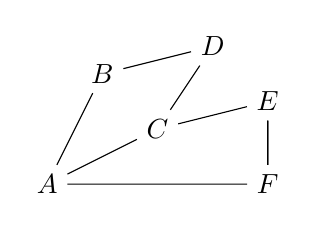
\begin{tikzpicture}[scale=.7]
  \node (A) at (-1,0) {$A$};
  \node (B) at (0,2) {$B$};
  \node (C) at (1,1) {$C$};
 \node (E) at (3,1.5) {$E$};
 \node (F) at (3,0) {$F$};
 \node (D) at (2,2.5) {$D$};
  \draw (C)--(A)--(B)--(D)--(C) --(E)-- (F); 
  \draw (A)--(F)--(E);
\end{tikzpicture}
$$

\end{example}


\begin{definition}{Relacja liniowo porządkująca (liniowy porządek) \cite[Rozdział 2]{blaszczyk2007}}\label{def-porzadek-liniowy}
Niech dany będzie niepusty zbiór $X$. Relację $\leq$ porządkującą zbiór $X$, nazywamy relacją liniowo porządkującą lub porządkiem liniowym, gdy dla dowolnych $x$, $y \in X$ spełnia ona następujący warunek spójności tzn.

$x \leq y$ lub $y \leq x$

Parę $(X, \leq)$ nazywamy zbiorem liniowo uporządkowanym lub łańcuchem.
\end{definition}


\begin{definition}{Dobry porządek \cite[Rozdział 2]{blaszczyk2007}}
Niech dany będzie zbiór $X$. Relację $\leq$ porządkującą zbiór $X$, nazywamy dobrym porządkiem na zbiorze $X$, gdy w każdym niepustym podzbiorze zbioru $X$ istnieje element najmniejszy względem relacji $\leq$. Jeśli relacja $\leq$ na zbiorze $X$ jest dobrym porządkiem, to mówimy, że para $(X,\leq)$ jest zbiorem dobrze uporządkowanym.
\end{definition}

\begin{definition}{Elementy wyróżnione \cite[Rozdział 2]{blaszczyk2007}}
Niech $X$ będzie zbiorem częściowo uporządkowanym przez relacje $\leq$ oraz niech $a \in X$. Mówimy, że:
\begin{enumerate}
\item $a$ jest elementem najmniejszym w $X$, gdy $\forall x \in X \quad a \leq x$
\item $a$ jest elementem minimalnym w $X$, gdy $\lnot ((\exists x \in X) \quad x <a )$
\item $a$ jest elementem największym w $X$, gdy $\forall x \in X \quad x\leq a$
\item $a$ jest elementem maksymalnym w $X$, gdy $\lnot ((\exists x\in X) \quad a <x)$
\end{enumerate}

\end{definition}


\begin{definition}{Ograniczenie górne \cite[Rozdział 2]{blaszczyk2007}}
Niech $A \subseteq X$, gdzie $(X, \leq)$ jest zbiorem uporządkowanym. Element $x \in X$ nazywamy ograniczeniem górnym zbioru $A$ względem relacji $\leq$, gdy $a \leq x$ dla każdego $a \in A$. 
\end{definition}


\begin{definition}{Ograniczenie dolne \cite[Rozdział 2]{blaszczyk2007}}
Niech $A \subseteq X$, gdzie $(X, \leq)$ jest zbiorem uporządkowanym. Element $y \in X$ nazywamy ograniczeniem dolnym zbioru $A$ względem relacji $\leq$, gdy $y \leq a$ dla każdego $a \in A$. 
\end{definition}


\begin{definition}{Zbiór ograniczony z góry, zbiór ograniczony z dołu, zbiór ograniczony \cite[Rozdział 2]{blaszczyk2007}}
Niech $A \subseteq X$, gdzie $(X, \leq)$ jest zbiorem uporządkowanym. Zbiór nazywamy ograniczonym z góry (ograniczonym z dołu), jeśli ma on ograniczenie górne (dolne). 
$\newline$ 
Zbiór ograniczony z dołu i z góry nazywamy ograniczonym. 
\end{definition}


\begin{definition}{Kres górny \cite[Rozdział 2]{blaszczyk2007}}
Niech $A \subseteq X$, gdzie $(X, \leq)$ jest zbiorem uporządkowanym. Jeśli zbiór $A$ jest ograniczony z góry i wśród ograniczeń górnych zbioru $A$ istnienie element najmniejszy $x_0$, to element ten nazywamy kresem górnym zbioru $A$ i oznaczamy symbolem $sup A$. Tak więc $x_0 =sup A$, gdy spełnione są następujące warunki:
\begin{enumerate}
\item $a \leq x_0$ dla każdego $a \in A$,
\item jeśli $a \leq x$ dla każdego $a \in A$, to $x_0 \leq x$.
\end{enumerate}
\end{definition}


\begin{definition}{Kres dolnym \cite[Rozdział 2]{blaszczyk2007}}
Niech $A \subseteq X$, gdzie $(X, \leq)$ jest zbiorem uporządkowanym. Jeśli zbiór $A$ jest ograniczony z dołu i wśród ograniczeń dolnych zbioru $A$ istnienie element największy $x_0$, to element ten nazywamy kresem dolnym zbioru $A$ i oznaczamy symbolem $inf A$. Tak więc $x_0 =inf A$, gdy spełnione są następujące warunki:
\begin{enumerate}
\item $y_0 \leq a$ dla każdego $a \in A$,
\item jeśli $y \leq a$ dla każdego $a \in A$, to $y \leq y_0$.
\end{enumerate}
\end{definition}


\begin{definition}{Zbiory równoliczne \cite[Rozdział 5]{blaszczyk2007}}
Mówimy, że zbiory $A$ i $B$ są równoliczne (tej samej mocy), gdy istnieje bijekcja, tj. funkcja $f$ różnowartościowa, przekształcająca zbiór $A$ na zbiór $B$, tzn. $f: A \rightarrow B$. Piszemy wtedy:  $\licznosc{A}=\licznosc{B}$.
\end{definition}


\begin{definition}{Zbiór skończony \cite[Rozdział 5]{blaszczyk2007}}
Mówimy, że zbiór $A$ jest skończony, gdy jest pusty lub równoliczny ze zbiorem $\{1, \ldots, n \}$, dla pewnego $n \in \mathbb{N}$. Gdy zbiór jest równoliczny ze zbiorem $\{1, \ldots, n\}$, to mówimy że jest on $n$-elementowy, tj. mocy równej $n$.
%Mówimy, że zbiór $A$ jest skończony, gdy istnieje taka $n \in \mathbb{N} \cup \{0\}$, że zbiór $A$ jest równoliczny z przedziałem w zbiorze liczb naturalnych
%\begin{center}
%$[0, n) = \{ k \in \mathbb{N}: k < n\}.$
%\end{center}
%Zatem, gdy zbiór $A$ jest równoliczny ze zbiorem $\{1, ..., k\}$, to mówimy że jest on $k$-elementowy, tj. %mocy równej $k$.
\end{definition}


\begin{definition}{Zbiór przeliczalny \cite[Rozdział 5]{blaszczyk2007}}
Mówimy, że zbiór $X$ jest przeliczalny, gdy jest skończony lub jest równoliczny z $\mathbb{N}$.
\end{definition}


%NA PODSTAWIE https://edu.pjwstk.edu.pl/wyklady/mad/scb/mad10/main10_p4.html
%to:
%Zbiory $A$ i $B$ nazywamy równolicznymi (tej samej mocy), jeśli istnieje pewna funkcja $f$ przekształcająca wzajemnie i jednoznacznie zbiór $A$ na zbiór $B$. Piszemy wtedy: $\licznosc{A}=\licznosc{B}$.




\subsection{Przestrzenie metryczne, miary odległości}


Niezbędnym jest również wprowadzenie podstawowych pojęć z topologii, ze względu na stosowanie funkcji odległości w celu uporządkowania obiektów.


\begin{definition}{Metryka \cite[Rozdzial 9]{kuratowski2004}}
Niech $X$ będzie niepustym zbiorem, wtedy funkcję $\mathrm{d}: X \times X \rightarrow [0,\infty)$, nazywamy metryką jeśli spełnione są warunki:
\begin{enumerate}
\item $\forall x, y \in X \quad \big(\mathrm{d}(x,y) = 0  \Longleftrightarrow x=y \big)$,
\item $\forall x, y \in X \quad \mathrm{d}(x,y)=\mathrm{d}(y,x)$,
\item $\forall  x, y, z \in X \quad \mathrm{d}(x,y)\leq \mathrm{d}(x,z)+\mathrm{d}(z,y)$.
\end{enumerate}
%Parę $\(X,\mathrm{d})$ nazywamy przestrzenią metryczną.
\end{definition}


\begin{definition}{Przestrzeń metryczna \cite[Rozdział 9]{kuratowski2004}}
Niech $X$ będzie niepustym zbiorem, $\mathrm{d}$ metryką, wówczas parę $(X,\mathrm{d})$ nazywamy przestrzenią metryczną. 
\end{definition}


\begin{example}{Metryka euklidesowa w $\mathbb{R}^2$}
Niech $\mathrm{d}_e: \mathbb{R}^2 \times \mathbb{R}^2 \rightarrow \mathbb{R}$ będzie metryką euklidesową, wówczas
$$\forall{(x_{1},x_{2}),(y_{1},y_{2}) \in \mathbb{R}^2} \quad \mathrm{d}_e((x_1,y_1),(x_2,y_2)):= \sqrt{(x_2-x_1)^2+(y_2-y_1)^2}. $$
%Niech $x=(x_1,x_2)$ oraz $y=(y_1,y_2)$, wówczas 
%\begin{center}
%$\mathrm{d}_e((x_1,y_1),(x_2,y_2)):= \sqrt{(x_2-x_1)^2+(y_2-y_1)^2}.$\\
%\end{center}
\end{example}


\begin{example}{Metryka miejska(Manhattan) w $\mathbb{R}^2$}
Niech $\mathrm{d}_m: \mathbb{R}^2 \times \mathbb{R}^2 \rightarrow \mathbb{R}$ będzie metryką miejską, wówczas 

$$\forall{(x_{1},x_{2}),(y_{1},y_{2}) \in \mathbb{R}^2} \quad \mathrm{d}_m((x_1,y_1),(x_2,y_2)):=|x_1-x_2|+|y_1-y_2|.$$

\end{example}


\begin{example}{Przestrzeń euklidesowa $n$-wymiarowa $\mathbb{R}^n$}
Niech $\mathrm{d}_e: \mathbb{R}^n \times \mathbb{R}^n \rightarrow \mathbb{R}$ będzie metryką euklidesową, wówczas
$$\forall{(x_1,x_2,\ldots,x_n),(y_1,y_2,\ldots,y_n) \in \mathbb{R}^n} \quad \mathrm{d}_e(x,y):= \sqrt{\sum_{i=1}^{n} |x_i-y_i|^2}.$$
\end{example}

%Tw o metryce euklidesowej w K^n ?? -zeszyt topologia rok 2 

\subsection{Rachunek macierzowy}

\begin{definition}{Grupa \cite[Rozdział 0]{banaszak2002}}
Grupą nazywamy zbiór P z działaniem $\cdot: P \times P \rightarrow P$ dla którego są spełnione następujące warunki:
\begin{enumerate}
\item Dla dowolnych $a,b,c \in P \quad (a\cdot b)\cdot c=a \cdot(b\cdot c) $ (łączność)
\item Istnieje element $e \in P$ (nazywany elementem neutralnym grupy), taki że dla każdego $a \in P$ mamy, $e\cdot a=a\cdot e=a$
\item Dla każdego $a \in P$ istnieje element $b\in P$ (nazywany elementem odwrotnym do $a$), taki że $a\cdot b=b \cdot a=e$.
\end{enumerate}
Dodatkowo, mówimy że grupa $P$ jest przemienna, gdy dla dowolnych $a,b\in P \quad a\cdot b=b\cdot a$.
\end{definition}

\begin{definition}{Pierścień \cite[Rozdział 0]{banaszak2002}}
Pierścieniem nazywamy zbiór $R$ z dwoma działaniami: z dodawaniem $+: R\times R \rightarrow R$ i z mnożeniem $\cdot: R \times R \rightarrow R$, dla których są spełnione następujące warunki:
\begin{enumerate}
\item Zbiór $R$ z działaniem $+$ jest grupą przemienną. Element neutralny działania $+$oznaczamy przez 0.
\item Dla dowolnych $a,b,c \in R \quad (a\cdot b)\cdot c=a\cdot(b\cdot c)$ (łączność mnożenia).
\item Dla dowolnych $a, b,c \in R$
$$
a \cdot (b+c)=a\cdot b + a\cdot c
$$
$$
(a+b) \cdot c=a\cdot c + b\cdot c
$$(rozdzielność mnożenia względem dodawania).
\end{enumerate}

\end{definition}

\begin{definition}{Ciało \cite[Rozdział 0]{banaszak2002}}
Ciałem nazywamy zbiór $K$ z działaniami: $+: K\times K \rightarrow K$ oraz $\cdot: K \times K \rightarrow K$, takimi że:
\begin{enumerate}
\item Zbiór $K$ z działaniami $+$ i $\cdot$ jest pierścieniem przemiennym z jedynką.
\item Zbiór $K^{*}=K \backslash \{0\}$ z działaniem $\cdot$ jest grupa.
\end{enumerate}
\end{definition}

\begin{definition}{Macierz \cite[Rozdział 1]{banaszak2002}}
Niech $K$ będzie ciałem i $m, n \in \mathbb{N}$. Macierzą o $m$-wierszach, $n$-kolumnach i o wyrazach z $K$ nazywamy każdą funkcję postaci
$A: \{1,\ldots, m \} \times \{1, \ldots, n\} \rightarrow K$
\end{definition}

\begin{example}
Macierz $A$ o $m$-wierszach i $n$-kolumnach najczęściej zapisuje się postaci $A= [a_{ij}]_{i \leq m, j \leq n}$, tj. 
$$
A= \begin{bmatrix}
a_{11} & a_{12} &  & a_{1n} \\
a_{21} & a_{22} & \ldots & a_{2n}\\ 
\ldots & \ldots & \ldots & \ldots\\
a_{m1} & a_{m2} & \ldots & a_{mn} \\
\end{bmatrix}    
$$
\end{example}



\chapter{Metody porządkowania}\label{metody porzadkowania}
Rozdział ten został opracowany w oparciu o \cite[Rozdział 2]{panek2013}, omówiono w nim ogólnie wybrane metody porządkowania zarówno liniowego jak i nieliniowego, po to by w kolejnym rozdziale szczegółowo przyjrzeć się wybranym metodą wraz z przedstawieniem ich algorytmów oraz dokładnych opisów matematycznych, z uwzględnieniem ich wad oraz zalet.

Metody porządkowania liniowego umożliwiają przeprowadzenie takiego porządkowania, w wyniku którego kolejność obiektów zwracana jest od tego o najlepszych zmiennych do tego o najsłabszych zmiennych, które opisują obiekt, innymi słowy ustalana jest hierarchia obiektów, na podstawie określonego kryterium(np. wartości zmiennych). Z kolei metody porządkowania nieliniowego nie pozwalają na ustaleniu hierarchii, natomiast w wyniku uporządkowania możliwe jest wskazanie dla każdego z obiektów poddanych porządkowaniu, obiektów podobnych ze względu na opisujące je zmienne. 
 %Problematyka związana z grupowaniem obiektów ma tutaj znaczenie drugoplanowe. Natomiast stosowanie metod porządkowania nieliniowego nie pozwala na ustalenie hierarchii obiektów, lecz wyłącznie wskazanie dla każdego z tych obiektów podobnych ze względu na wartości opisujących je zmiennych. Powoduje to, że porządkowanie nieliniowe stanowi przede wszystkim etap wstępny do grupowania obiektów.\\

\section{Metody porządkowania liniowego}

W wielowymiarowej przestrzeni zmiennych, porządkowanie liniowe obiektów sprowadza się do rzutowania punktów na prostą, przy czym punkty reprezentują obiekty poddane porządkowaniu. Taka operacja pozwala ustalenie hierarchii obiektów - o czym z resztą wspomniałam już na początku tego rozdziału.
Poniżej zostaną przedstawione własności uporządkowania liniowego obiektów, wraz z podaniem ich matematycznej interpretacji.

\begin{itemize}
\item każdy obiekt ma przynajmniej jednego sąsiada i nie więcej niż dwóch sąsiadów,
\item jeżeli sąsiadem $i$-tego obiektu jest $k$-ty obiekt, to jednocześnie sąsiadem $k$-tego obiektu jest $i$-ty obiekt,
\item dokładnie dwa obiekty mają tylko jednego sąsiada.
\end{itemize}


Powyżej wymienione własności są wynikiem posiadania jedynie skończonej ilości obiektów, które podane są uporządkowaniu. W następnej części chciałabym 
\begin{itemize}
\item sformalizować rozumienie powyższych własności,
\item udowodnić ich poprawność,
\item rozważyć dostateczność tych własności w zbiorach o skończonej ilości obiektów.
\end{itemize}


Na początku zacznę od sprecyzowania takich pojęć jak sąsiad względem relacji.

\begin{definition}{Sąsiad względem relacji $\leq$}\label{def-sasiada}
Niech  $X$ będzie niepustym zbiorem, a $x, y$ będą dwoma różnymi elementami należącymi do tego zbioru. Mówi się, że $y \in X$ jest sąsiadem $x \in X$,co zapisujemy $ySx$, jeśli

$\left(y \leq x \lor x \leq y \right) \quad \land \quad  \left(\lnot \exists_{z \in X}  \quad x\neq z \neq y \Rightarrow   y \leq z \leq x \lor x \leq z \leq y \right)$.

\end{definition}


\begin{theorem}{Własności porządku liniowego w zbiorach skończonych}
Niech $\leq$ będzie relacją porządku liniowego zdefiniowaną w $X \times X$, gdzie $X$ jest zbiorem ze skończoną liczbą obiektów, złożonym co najmniej z dwóch elementów. Wtedy
\begin{enumerate}
\item $\forall_{x \in X} \quad \licznosc{\{y \in X, ySx\}} \in \{1,2\}$,
\item $\forall_{x, y \in X} \quad ySx \Rightarrow xSy $,
\item $\licznosc{\{x \in X, \quad \licznosc{\{y \in X, \quad ySx \}}=1\}}=2$
\end{enumerate}
gdzie $S$ oznacza sąsiada względem relacji $\leq$.
\end{theorem}


\begin{proof}
Poniżej zostaną udowodnione powyższe własności.
\begin{enumerate}
\item Niech $x \in X$. Przypuśćmy na początek, że $\licznosc{\{y \in X, ySx\}} = 0$, tzn. że obiekt $x$ nie posiada sąsiadów w tej relacji. Nasz zbiór $X$ jest jednak co najmniej dwuelementowy zatem istnieje element $y \in X$ i $ x \neq y$. Wobec spójności linowego porządku z Definicji \ref{def-porzadek-liniowy} zachodzi wtedy
$$ x \leq y \lor y \leq x.$$
Jednak wiemy, że $y$ nie może być sąsiadem $x$ gdyż ten nie posiada sąsiadów. Zatem z definicji sąsiada musi istnieć $z \in X$ różny od obu $x \neq z \neq y$ spełniający warunek
$$
z \leq x \lor x \leq z.
$$
Powyższe rozumowanie dla $y$ można by dalej zastosować do $z$, uzyskując kolejne $z_1$ a później $z_2,z_3, \ldots$ dowolną ilość różnych elementów z których każdy występuje w relacji liniowego porządku z $x$, ale żaden z nich nie jest sąsiadem. Jednak nasz zbiór $X$ jest zbiorem skończonym, więc nigdy nie uda nam się utworzyć dowolnej ilości różnych elementów ze zbioru $X$ (elementy się wyczerpią). Zatem nasze przypuszczenie, że $\licznosc{\{y \in X, ySx\}} = 0$ jest fałszywe.

Przypuśćmy dalej, że $\licznosc{\{y \in X, ySx\}} \geq 3$. Niech $a,b,c$ będą trzema różnymi elementami z $X$ będącymi sąsiadami dla $x$. Wtedy bez straty ogólności możemy przyjąć, że $a \leq x, b \leq x$ lub $x \leq a, x \leq b$. Istotnie mając 3 elementy w relacji wtedy co najmniej dwa muszą znajdować się po zgodnej stronie, a z dokładnością do oznaczeń możemy przyjąć, że będą nimi $a$ oraz $b$. Ustalmy zatem, że $a \leq x, b \leq x$. Wobec definicji \ref{def-porzadek-liniowy} wiemy, że $a \leq b$ lub $b \leq a$. Jeśli $a \leq b$ to $a \leq b \leq x$. Co przeczy temu, że $a$ jest sąsiadem $x$. Jeśli $b \leq a$ to $b \leq a \leq x$ co przeczy temu, że $b$ jest sąsiadem. Zupełnie analogicznie postępujemy dla przypadku $x \leq a, x \leq b$. Zatem uzyskujemy sprzeczność, będącą efektem przypuszczenia, że mogą istnieć takie 3 elementy $a,b,c$. Zatem ostatecznie $\licznosc{\{y \in X, ySx\}} \in \{ 1,2 \}$.

\item Niech $x,y \in X$ oraz niech $ySx$. Korzystając z definicji sąsiada \ref{def-sasiada} mamy, że skoro $ySx$ to  $$\left(y \leq x \lor x\leq y \right)\quad \land \quad  \left(\lnot \exists_{z \in X}  \quad x\neq z \neq y \Rightarrow   y \leq z \leq x \lor x \leq z \leq y \right),$$ Natomiast $xSy$ oznacza, że $$\left(x \leq y \lor y\leq x \right)\quad \land \quad  \left(\lnot \exists_{z \in X}  \quad y\neq z \neq x \Rightarrow   x \leq z \leq y \lor y \leq z \leq x \right).$$ 
Wobec powyższego widać, że te dwa zdania znaczą to samo, stąd widać że  $ySx \Rightarrow xSy$. %spojnosc nie pokazywala ze to z moze istniec miedzy x i y

\item Intuicyjnie te dwa elementy posiadające po jednym sąsiedzie są elementami maksymalnym i minimalnym w tym zbiorze. Udowodnimy kolejno:
\begin{itemize}
\item Element minimalny w zbiorze ma pojedynczego sąsiada. Załóżmy, że zbiór musi posiadać dokładnie 1 element minimalny, tzn. $x_m \in X$ takie, że 
$$
\forall x \in X \quad x_m \leq x.
$$
Istotnie przypuśćmy, że nie istnieje element minimalny. Niech $x_1$ będzie dowolnym elementem z $X$. Skoro nie istnieje element minimalny, to istnieje $x_2 \in X$ takie, że $x_2 \leq x_1$ i $x_2 \neq x_1$. Dla $x_2$ z braku elementu minimalnemu, musi istnieć z kolei $x_3 \leq x_2$ takie, że $x_2 \neq x_3$. Itd. Co nie jest możliwe, gdyż zbiór $X$ jest przecież skończonym zbiorem.
Rozważmy dalej przypuszczenie gdyby były dwa lub więcej takich elementów. Wtedy to, z antysymetryczności, oczywiście musiałyby być sobie równe. Jeśli $x_m, y_m$ są jednocześnie minimalne to
$$
\forall x \in X \quad x_m \leq x,
$$
oraz 
$$
\forall x \in X \quad y_m \leq x.
$$
Skąd natychmiast mamy, że $ x_m \leq y_m$ oraz $y_m \leq x_m$. Wobec antysymetryczności z definicji \ref{def-relacja-czesciowego-porzadku} mamy, że $x_m = y_m$ wbrew naszemu przypuszczeniu, że są od siebie różne.
Pozostaje pokazać, że element minimalny ma pojedynczego sąsiada. Przypuśćmy, że $y,z \in X$ są dwoma różnymi sąsiadami dla $x_m$. Wtedy $ x_m \leq y \lor y \leq x_m$ oraz $ x_m \leq z \lor z \leq x_m$. Skoro $x_m$ jest minimalny to musi to oznaczać, że
$$
x_m \leq y \land x_m \leq z.
$$ 
Wobec spójności z definicji \ref{def-porzadek-liniowy} zachodzi $y \leq z$ lub $z \leq y$. Sprzeczność, gdyż wtedy któryś z nich nie mógłby być sąsiadem dla $x_m$.
\item Element maksymalny $x_M$ w zbiorze ma pojedynczego sąsiada. Analogicznie do powyższego punktu, zbiór musi posiadać dokładnie 1 element maksymalny, tzn. $x_M \in X$ takie, że
$$\forall x \in X \quad x \leq x_M.$$
Istotnie przypuśćmy, że nie istnieje element maksymalny. Niech $x_1$ będzie dowolnym elementem z $X$. Skoro nie istnieje element maksymalny, to istnieje $x_2 \in X$ takie, że $x_1 \leq x_2$ i $x_1 \neq x_2$. Dla $x_2$ z braku elementu maksymalnego, musi istnieć taki element $x_3 \in X$ i $x_3 \neq x_2$, że $x_2 \leq x_3$. Itd. Co nie jest możliwe, gdyż z założenia, zbiór $X$ jest skończonym zbiorem.
Rozważmy dalej przypuszczenie gdyby były dwa lub więcej takich elementów. Wtedy to, z antysymetryczności, musiałyby być sobie równe. Jeśli $x_M, y_M$ są jednocześnie maksymalne, to 
$$
\forall x \in X \quad x \leq x_M,
$$
oraz 
$$
\forall x \in X \quad x \leq y_M.
$$
Stąd natychmiast mamy, że $x_M \leq y_M$ oraz $y_M \leq  x_M$. Wobec antysymetryczności z definicji \ref{def-relacja-czesciowego-porzadku}, mamy że $x_M = y_M$, co wbrew naszemu przypuszczeniu daje, że elementy te nie są od siebie różne.
Pozostaje pokazać, że element maksymalny ma pojedynczego sąsiada. Przypuśćmy, że $y, z \in X$ są dwoma różnymi sąsiadami dla $x_M$. Wtedy $ x_M \leq y \lor y \leq x_M$ oraz $ x_M \leq z \lor z \leq x_M$. Skoro $x_M$ jest elementem maksymalny to musi to zatem oznaczać
$$
y \leq x_M \land z \leq x_M.
$$ 
Wobec spójności z definicji \ref{def-porzadek-liniowy} zachodzi $y \leq z$ lub $z \leq y$. Sprzeczność, gdyż wtedy któryś z nich nie mógłby być sąsiadem dla $x_M$.

\item Żaden inny element nie może mieć pojedynczego sąsiada. Przypuśćmy, że $x \in X$ nie będąc ani elementem minimalnym ani maksymalnym ma pojedynczego sąsiada. Wobec definicji elementu minimalnego i maksymalnego oraz spójności zachodzi
$$
x_m \leq x \leq x_M.
$$
Zatem albo $x_m$ jest sąsiadem $x$ albo istnieje $y_1 \in X$ taki, że $y_1 \leq x$.
Tworzy to kilka możliwych przypadków. W pierwszym $x_m$ będzie tym jedynym sąsiadem, w drugim $x_M$ nim będzie, w ostatnim natomiast, ani $x_m$, ani $x_M$ nie będą sąsiadami.

Zajmiemy się najpierw pierwszym z nich, tj. $x_m$ jest sąsiadem $x$. Zauważmy teraz, że z faktu, iż $x_M$ jest elementem maksymalnym zbioru $X$, wynika że $ x \leq x_M$. Nie jest jednak sąsiadem elementu $x$. Zatem istnieje takie $x_1 \in X$, że $x\leq x_1 \leq x_M$. Jednak $x_1$ również nie może być sąsiadem $X$ co powoduje, że istnieje taki element $x_2 \in X$, że $x \leq x_2 \leq x_1 \leq x_M$. Itd. Jednakże, skoro zbiór $X$ jest zbiorem skończonym, to musi istnieć taki element $x_j \in X$, że $x \leq x_j$, który będzie sąsiadem z $x$, zatem $xSx_j$. Zatem ostatecznie $xSx_m$ i $xSx_j$, a to przeczy założeniu, że $x$ ma pojedynczego sąsiada. 

Przejdźmy teraz do drugiego przypadku, tj. gdy $x_M$ jest sąsiadem dla $x$. Wtedy $x_m$ nie jest sąsiadem dla $x$ jednak wiedząc, że $x_m \leq X$ musi istnieć $y_1\in X$, taki że $y_1 \leq x$. Jednak wiedząc iż $y_1$ nie jest sąsiadem dla $X$ wnioskujemy, że istnieje taki $y_2 \in X$, że $x_m \leq y_1 \leq y_2 \leq x$. Itd.  Jednakże, skoro zbiór $X$ jest zbiorem skończonym, to musi istnieć taki element $y_i \in X$, że $y_i \leq x$, który będzie sąsiadem z $x$. Zatem ostatecznie $y_iSx$ i $xSx_M$, co przeczy założeniu że $x$ ma pojedynczego sąsiada.

Zajmijmy się teraz trzecim przypadkiem, tj. gdy ani $x_m$ oraz $x_M$ nie są sąsiadami elementu $x$. Z faktu, iż zbiór $X$ posiada element minimalny $x_m$, który nie jest sąsiadem elementu $x$, wynika że istnieje taki element $x_1 \in X$, że $x_m \leq x_1 \leq x$. Co więcej istnieje taki $x_2 \in X$, że $x_m \leq x_1 \leq x_2 \leq x.$ Itd. I znów skoro zbiór $X$ jest skończony, to istnieje taki element $x_j \in X$, że $x_j \leq x$ i $x_jSx$. Z drugiej strony, skoro zbiór $X$ posiada element maksymalny $x_M$, który nie jest sąsiadem elementu $x$, wynika że istnieje taki element $y_1 \in X$, że $x \leq y_1 \leq x_M$. Analogicznie do wcześniejszych kroków, istnieje takie element $y_2 \in X$, że $x \leq y_2 \leq y_1 \leq x_M$. Itd.  Zbiór $X$ jest zbiorem skończonym, zatem musi istnieć taki element $y_i \in X$, że $x \leq y_i$ i $xSy_1$. 
Łącząc te dwa warunki, wynika że $x$ musi mieć dwóch sąsiadów. Co kończy dowód własności.

\end{itemize}

\end{enumerate}
\end{proof}

Powyżej wykazane własności są często podawane, niemal na równi z definicją takiego uporządkowania, w pozycjach książkowych omawiających praktyczny aspekt porządkowania danych. Poniżej podane zostaną przykłady takich relacji, które też posiadają powyższy zestaw własności, ale nie opisują relacji będących porządkami liniowymi. 
 
\begin{example}
Rozważmy zbiór dwuelementowy $X = \{ a, b \}$ gdzie $a \leq b$ jest jedynym punktem tej relacji. Tak zdefiniowana relacja spełnia wszystkie własności, ale nie spełnia założenia o zwrotności - zatem relacja ta nie jest liniowym porządkiem. 

Diagram Hassego prezentujący tę relację, jest postaci: 
$$
\begin{tikzpicture}[scale=.7]
  \node (a) at (-2,0) {$a$};
  \node (b) at (2,1) {$b$};
%  \node (zero) at (0,-2) {$0$};
  \draw (a)--(b) ; %-- (one) -- (d) -- (zero);
\end{tikzpicture}
$$
\end{example}

\begin{example}
Rozważmy zbiór $X = \{a,b,c,d,e \}$ oraz relację definiującą następujące sąsiedztwa (wypisaną bez par symetrycznych) $aSb, bSc, aSc, dSe$. Ponadto dołóżmy warunek zwrotności, tj. $a \leq a$, $b \leq b$, $c \leq c$, $d \leq d$, $e \leq e$. 

Diagram Hassego prezentujący relację porządku tego zbioru, jest postaci:
$$
\begin{tikzpicture}[scale=.7]
  \node (a) at (-2,0) {$a$};
  \node (b) at (2,0) {$b$};
  \node (c) at (2,2) {$c$};
 \node (e) at (1,3) {$e$};
 \node (d) at (-3,3) {$d$};
%  \node (zero) at (0,-2) {$0$};
  \draw (b)--(a) --(c)-- (b) -- (c); %--(e)--(d); -- (one) -- (d) -- (zero);
  \draw (d)--(e);
\end{tikzpicture}
$$
%https://tex.stackexchange.com/questions/47392/how-to-draw-a-poset-hasse-diagram-using-tikz
%https://tex.stackexchange.com/questions/129583/how-can-i-produce-a-hasse-or-lattice-diagram/129641
Z diagramu widać, że taka relacja spełnia wszystkie omawiane wcześniej własności - jednak nie jest spójna. I tak np. nie możemy porównać elementów $a$ i $d$, bowiem nie możemy określić czy  $d \leq a$ lub $a \leq d$.
\end{example}

%przyklady diagramow hassego!!! https://www.math.uni.wroc.pl/~newelski/dydaktyka/wdm-A/skrypt3/skrypt/node9.html


W podsumowaniu tej sekcji należy podkreślić, że by uporządkować liniowo obiekty, charakteryzujące je zmienne muszą być mierzone przynajmniej na skali porządkowej. Istotne jest również aby miały jednakowy charakter, na potrzeby pracy zakładam, że zmiennej opisujące obiekty powinny być stymulantami, gdy nimi nie są należy dokonać stymulacji. Operacja ta umożliwia w dalszym kroku przejścia do transformacji normalizacyjnej, która konieczna jest gdy zmienne opisujące obiekty mierzone są na skali przedziałowej lub ilorazowej, a chcemy uzyskać ich porównywalność.
% W przypadku, gdy zmienne mierzone są na skali przedziałowej lub ilorazowej, należy dokonać ich normalizacji, dla zapewnienia ich porównywalności.

Metody porządkowania liniowego można podzielić na metody diagramowe, procedury oparte na zmiennej syntetycznej oraz procedury iteracyjne bazujące funkcji kryterium dobroci uporządkowania tzn. funkcji, którą się przyjmuje, lub też tworzy się ją aby w kolejnych iteracjach szukać takiego uporządkowania, które optymalizuje zbiór wartości tej funkcji. W kolejnej sekcji zostaną pokrótce przedstawione różne metody, z wyszczególnieniem najważniejszych założeń każdej z nich.


\subsection{Metody diagramowe}


W metodach diagramowych stosuje się graficzną reprezentację macierzy odległości zwanej diagramem. Macierz konstruowana jest w oparciu o odległości między obiektami, wyznaczone za pomocą dowolnej metryki. Porządkowanie obiektów polega na porządkowaniu diagramu, tj. przestawieniu wierszy i odpowiadających im kolumn, w celu by wzdłuż przekątnej skupiały się najmniejsze odległości zaś im dalej od głównej przekątnej tym większe odległości między zmiennymi opisującymi porządkowane obiekty.  %tak aby symbole graficzne reprezentujące najmniejsze odległości skupiały się wzdłuż głównej przekątnej, zaś w miarę oddalania się od głównej przekątnej znajdowały się symbole graficzne odpowiadające coraz to większym odległością.  %W kolejnym etapie następuje dzielenie mierników odległości macierzy, na klasy podobieństwa obiektów. Kolejny krok polega na przyporządkowaniu poszczególnym klasom podobieństwa, obiektów odpowiedniego symbolu graficznego. Samo porządkowanie obiektów polega na porządkowaniu diagramu, tj. przestawieniu wierszy i odpowiadających im kolumn diagramu, tak aby symbole graficzne reprezentujące najmniejsze odległości skupiały się wzdłuż głównej przekątnej, zaś w miarę oddalania się od głównej przekątnej znajdowały się symbole graficzne odpowiadające coraz to większym odległością. 

Jako narzędzie pomocnicze w porządkowaniu danych, może stanowić kryterium postaci:


$$
F^1= \sum_{i=1}^{n} \sum_{k>1}^{n} d_{ik}w_{ik}
$$

gdzie:

 $d_{ik}$ - odległość euklidesowa między $i$-tym i $k$-tym obiektem . 
 
 $w_{ik}$ - wagi elementów macierzy odległości, zdefiniowane w oparciu o jeden z następujących wzorów: 
 
$$
w_{ik}=\frac{| i-k |}{n-1}, \qquad
$$

$$
w_{ik}=\frac{1}{n(n-1)}\lbrack{2n|i-k-1|+i+k-(i-i)^2\rbrack},
$$
$$
w_{ik}=\frac{1}{n(n-1)}\lbrack{2n|i-k|+2-i-k-(i-i)^2\rbrack}.
$$
 


Dodatkowo wagi elementów macierzy odległości tworzą macierz wag postaci:

$W=\lbrack{w_{ik}\rbrack},\quad i,k=1, 2, \ldots, n.$


%%przyklad diagramu http://www.antropologia.uw.edu.pl/MaCzek/maczek.html



\subsection{Metody oparte na zmiennych syntetycznych}

W tym podrozdziale zostaną opisane metody porządkowania oparte na zmiennych syntetycznych, tj. funkcji wyznaczonej na podstawie wartości zmiennych opisujących obiekty, której wartości będą służyć do porządkowania zbioru. Metody oparte na zmiennych syntetycznych dzielimy na wzorcowe i bezwzorcowe. Poniżej zostaną one opisane szczegółowo, jednak wcześniej zostaną przedstawione wzory wyznaczające zmienną syntetyczną. 

\subsubsection{Sposoby wyznaczania zmiennej syntetycznej}
W pracy dla zachowania ogólności, przyjmuję że wszystkie zmienne opisujące obiekty mają jednakowe wagi, w związku z tym wzory służące do wyznaczenia zmiennej syntetycznej są postaci:
\begin{enumerate}
\item dla średniej arytmetycznej:

$$
s_{i}=\frac{1}{m} \sum_{j=1}^{m} n_{ij},  \quad i=1, 2, \ldots, n,
$$

\item dla średniej geometrycznej:

$$
s_{i}=\prod_{j=1}^{m} (n_{ij})^{\frac{1}{m}}, \quad i=1, 2, \ldots, n,
$$

\item dla średniej harmonicznej

$$
s_{i}=\big[\sum_{j=1}^{m} \frac{1}{n_{ij}}\big]^{-1} \cdot m, \quad i=1, 2, \ldots, n,
$$

\end{enumerate}
gdzie:
$s_{i}$ - wartość zmiennej syntetycznej w $i$-tym obiekcie,
%$w_{j}$ - waga $j$-tej zmiennej.



\subsubsection{Metody bewzorcowe}


W metodach tych zakładamy, że nie istnieje obiekt wzorcowy, czyli taki o najkorzystniejszych wartościach zmiennych ze względu na ustalone kryterium porządkowania. Porządkowanie dokonywane jest na podstawie wartości zmiennej syntetycznej, wyznaczonej dla każdego obiektu. 
%W metodach tych, unormowane wartości podanych zmiennych wejściowych są uśrednianie, przez przypisywanie im odpowiednich wag. 
%%%UWAGAposluguje sie uogolnieniem, nie korzystam z wag zmiennych, obiektow!!!!!
Poniżej zostaną omówione wybrane metody porządkowania bezwzorcowego.

\subsubsection{Metoda rang}


Metoda ta opiera się na normalizacji rangowej, w związku z tym zmienne poddane porządkowaniu, powinny być mierzone są na skali porządkowej. Dla każdego obiektu wyznacza się sumę przyporządkowanych mu rang ze względu na wszystkie zmienne. Na końcu obliczana jest wartość zmiennej syntetycznej, jako średniej wartości rang. W oparciu o tę wartość następuje porządkowanie obiektów, tj. im wartość zmiennej syntetycznej jest mniejsza tym wyżej w hierarchii znajduje się uporządkowany obiekt. Wzór na obliczenie wartości zmiennej syntetycznej: 
$$
s_{i}=\frac{1}{m}\sum_{j=1}^{m} n_{ij},\quad i=1, 2, \ldots, n,
$$

gdzie:

$n_{ij}$-zmienna znormalizowana rangowo, tj.
$
n_{ij}=r$ dla $x_{rj}=x_{ij}, \quad h,i=1, 2, \ldots, n.
$
gdzie:

$r$-ranga nadana $i$-temu obiektowi znajdującemu się na $r$-tym miejscu w uporządkowanym szeregu obiektów ze względu na $j$-tą zmienną.


\subsubsection{Metoda sum}


Metoda ta używana jest w momencie, gdy zmienne mierzone są na skali ilorazowej lub przedziałowej. W związku z tym tuż po stymulacji zmiennych, należy dokonać ich przekształcenia normalizacyjnego, dokonanego za pomocą unitaryzacji. W kolejnym kroku, dla każdego obiektu wyznaczana jest zmienna syntetyczna, jako średnia arytmetyczna wartości zmiennych przy przyjęciu jednakowych wag dla każdej zmiennej, jako średnia arytmetyczna wartości zmiennych.
Następnie muszą zostać wyeliminowane ujemne wartości zmiennej syntetycznej, do czego służy poniższe przekształcenie:
%Metoda ta bazuje na konstrukcji zmiennej syntetycznej przy pomiarze zmiennych na skali ilorazowej lub przedziałowej, w związku z tym w pierwszym kroku należy dokonać przekształcenia zmiennych przy pomocy unitaryzacji. Następnie dla każdego obiektu obliczana jest wartość zmiennej syntetycznej, jako średnia arytmetyczna wartości zmiennych przy przyjęciu jednakowych wag dla każdej zmiennej. Eliminowane są ujemne wartości zmiennej syntetycznej przy wykorzystaniu przekształcenia: 
$$
s_{i}'=s_{i}-\min\{s_i\}, \quad i=1, 2, \ldots, n.
$$

Końcowa postać zmiennej syntetycznej otrzymywana jest, przy wykorzystaniu normalizacji o postaci: %po przeprowadzeniu normalizacji według wzoru:
$$
s_{i}''=\frac{s_{i}'}{\max\{s_{i}'\}},\quad i=1, 2, \ldots, n.
$$
Powyższe przekształcenia ujednolicają zakres miary syntetycznej do przedziału [0, 1]. Im wyższa wartość zmiennej syntetycznej, tym wyżej w hierarchii znajduje się obiekt.%powodują unormowanie miary syntetycznej w przedziale [0,1]. Powyższa wielkość wykorzystywana jest do uporządkowania obiektów.


\subsubsection{Metoda wzorcowe}


W metodach tych zakłada się istnienie obiektu wzorcowego $P_{0}=[n_{0j}], \quad  j= 1,2,\ldots,m$, w którym znormalizowane zmienne wejściowe $n_{0j},  j= 1,2,\ldots,m$, będące współrzędnymi obiektu wzorcowego, przyjmują optymalne wartości, które to są ustalane na podstawie ogólnie przyjętych norm, subiektywnej opinii dotyczącej obserwowanego obiektu, lub też opinii ekspertów. Poszczególne metody różnią się sposobem wyznaczania obiektu wzorcowego, poniżej zostaną one przedstawione.

\subsubsection{Metoda Hellwiga}


W metodzie tej, obiekt wzorcowy wyznaczony jest na podstawie wystandaryzowanych zmiennych wejściowych. Współrzędnym obiektu wzorcowego przyporządkowuje się maksimum, gdy zmienne wejściowe są stymulantami lub minimum gdy zmienne są destymulantami. Obiekty są uporządkowywane na podstawie odległości od obiektu wzorcowego, przy wykorzystaniu odległości euklidesowej.
Miara syntetyczna jest postaci: 
$$
s_i=1-\frac{d_{i0}}{d_{0}},\quad i=1, 2, \ldots, n ,
$$

gdzie:

$d_{i0}$-odległość $i$-tego obiektu, od obiektu wzorcowego

współrzędne obiektu wzorcowego są obliczane na podstawie wzoru:
$$n_{0j}=\left\{ \begin{array}{ll}
\max\limits_{i} \{n_{ij}\} & \textrm{dla  } n_{j}^S,\quad j=1,2,\dots,m, \quad i=1,2,\dots,n, \\
\min\limits_{i} \{n_{ij}\} & \textrm{dla } n_{j}^D, \quad j=1,2,\dots,m, \quad i=1,2,\dots,n,
\end{array} \right. $$
$$d_{i0}=\bigg[\sum_{j=1}^{m} (n_{ij} - z_{0j})^2 \bigg]^\frac{1}{2} ,$$ 
$$d_{0}=\overline{d_{0}} + 2S(d_{0}) ,$$
$$\overline{d_{0}}=\frac{1}{n}\sum_{i=1}^{n} d_{i0} ,$$
$$S(d_{0})=\bigg[\frac{1}{n}\sum_{i=1}^{n} (d_{i0}-\overline{d_{0}})^2 \bigg]^\frac{1}{2} .$$

Wartości miary $s_{i}$ zazwyczaj są z przedziału $[0, 1]$. Należy tu zaznaczyć, że wartości miary są tym wyższe, im mniej jest oddalony obiekt od obiektu wzorcowego. 

%\subsubsection{Metoda Walesiaka}
%
%
%Metoda ta bazuje na konstrukcji zmiennej syntetycznej w oparciu o badanie odległości obiektów od obiektu wzorcowego, przy wykorzystaniu uogólnionej miary odległości. Umożliwia ona  porządkowanie obiektów, jeżeli opisujące je charakterystyki są mierzone przynajmniej na skali porządkowej. W takim przypadku, zmienne wejściowe o postaci nominant muszą zostać podaje stymulacji. Z kolei gdy zmienne są mierzone na skali przedziałowej lub ilorazowej, należy je znormalizować. 
%Miara syntetyczna oparta na uogólnionej mierze odległości przyjmuje postać:
%\begin{equation}
%s_i=\frac{1}{2}-\frac{\sum_{j=1}^{m} w_{j}a_{i0j}b_{0ij} + \sum_{j=1}^{m}\sum_{i^{''}=1}^{n} w_{j}a_{ii^{''}j}b_{0i^{''}j}}{2\bigg[\bigg(\sum_{j=1}^{m}\sum_{i^{''}=1}^{n} w_{j}a^{2}_{ii^{''}j} \bigg)\cdot \bigg(\sum_{j=1}^{m}\sum_{i^{''}=1}^{n} w_{j}b^{2}_{0i^{''}j}\bigg) \bigg]^{\frac{1}{2} }}
%\end{equation}
%gdzie:
%\begin{itemize}
%\item $a_{ii^{*}j}$-miernik odległości $i$-tego obiektu o $j$-tej zmiennej, od  $i^{*}$-tego obiektu, gdzie $i^{*}=0,i^{''}$, przy czym $i^{''}\neq 0$
%\item $b_{0i^{*}j}$-miernik odległości obiektu wzorcowego o $j$-tej zmiennej, od $i^{*}$-tego obiektu, gdzie $i^{*}=i,i^{''}$, przy czym $i^{''}\neq 0$
%\item $w_{j}$-waga $j$ tej zmiennej, dla której spełnione są warunki:
%\end{itemize}
%$$w_{j} \in [0, m] \quad \land \quad \sum_{j=1}^{m} w_{j}=m$$
%
%
%Ostateczna postać zmiennej syntetycznej zależy od skali pomiaru zmiennych. 
%Jeśli zmienne charakteryzujące obiekty mierzone są na skali ilorazowej lub przedziałowej, stosowane jest następujące podstawienie:
%
%$a_{ii^{*}j}=n_{ij} - z_{i^{*}j}$ dla $i^{*}=0,i^{''},$
%
%$b_{0i^{*}j}=z_{0j}-z_{i^*j}$ dla $i^{*}=i,i^{''}$.
%
%gdzie:
%
%$z_{0j}$-wystandaryzowana wartość j-tej zmiennej dla obiektu wzorcowego
%
%
%Z kolei, gdy zmienne charakteryzujące obiekty mierzone są na skali porządkowej to stosowne jest podstawienie:
%\begin{equation}
%a_{ii^{*}j}=\left\{ \begin{array}{lll}
%1  & \textrm{dla  } n_{ij}>z_{i^{*}j}, \\
%0 & \textrm{dla } n_{ij}=z_{i^{*}j}, \quad i^{*}=0,i^{'},\\
%-1 & \textrm{dla } n_{ij}<z_{i^{*}j},\\
%\end{array} \right.
%\end{equation}
%
%\begin{equation}
%b_{0i^{*}j}=\left\{ \begin{array}{lll}
%1  & \textrm{dla  } z_{0j}>z_{i^{*}j}, \quad i^{*}=i,i^{'},\\
%0 & \textrm{dla } z_{0j}=z_{i^{*}j},\quad i^{*}=i,i^{'},\\
%-1 & \textrm{dla } z_{0j}<z_{i^{*}j}.\\
%\end{array} \right.
%\end{equation}
%Zmienna syntetyczna przyjmuje wartości z przedziału $[0,1]$. Czym niższa wartość zmiennej syntetycznej, tym bliżej wzorca leży dany obiekt.

\subsubsection{Metoda dystansowa}


Podobnie jak we wcześniejsze metodach, na początku zmienne należy poddać stymulacji, oraz przekształceniu normalizacyjnemu, wybranemu na podstawie skal do których należą zmienne opisujące obiekty. W kolejnym kroku wyznaczane są współrzędne obiektu wzorcowego, a następnie macierz odległości każdego obiektu od obiektu wzorcowego, w oparciu o nią wyznacza jest zmienna syntetyczna. Odległość od obiektu wzorca jest wyznaczana przy zastosowaniu dowolnej metryki, np. metryki euklidesowej. %W metodzie tej zmienna syntetyczna wyznaczana jest na podstawie odległości każdego obiektu od obiektu wzorca, przy wykorzystaniu np. metryki euklidesowej. 
Dla metody tej, miara syntetyczna jest wyznaczana za pomocą przekształcenia unitaryzacyjnego postaci: 

$$s_{i}=\bigg(\frac{d_{i0}-\min\limits_{i}\{d_{i0}\}}{\max\limits_{i}\{d_{i0}\}-\min\limits_{i}\{d_{i0}\}} \bigg)^{p}, \quad i=1,2,\dots,n \quad p \in \mathbb{N}
$$
Miara syntetyczna uzyskana tą metodą jest unormowana i przyjmuje wartości z przedziału: $[0,1]$. Czym niższa wartość miary, tym bliżej obiektu wzorcowego leży dany obiekt. 

\subsection{Metody iteracyjne}

%czym jest funkcja dobroci kryterium porządkowania - we wstepie rozdzailu gdzie opisano metody porzadkowania liniowego
W metodach tych przyjmowania jest funkcja kryterium dobroci porządkowania, dla której w kolejnych iteracjach poszukiwane jest takie uporządkowanie liniowe obiektów, które optymalizuje wartość funkcji kryterium, aż do osiągnięcia przez nią wartości optymalnej tj. maksymalnej lub minimalnej. 


\subsubsection{Metoda Szczotki}


Metoda ta polega na znalezieniu takiego uporządkowania liniowego obiektów, dla którego funkcja kryterium dobroci uporządkowania osiąga maksimum:
$$
F^{2}=\sum_{k=1}^{n-1} k\sum_{i=1}^{n-k} d_{ik} \rightarrow     \max  
$$
gdzie:

$d_{ik}$ - odległość euklidesowa miedzy $i$-tym i $k$-tym obiektem.

Sposób postępowania:

W pierwszym kroku przeprowadzane jest dowolne liniowe uporządkowanie obiektów. W kolejnym kroku, dla tego uporządkowania obliczana jest wartość funkcji kryterium dobroci uporządkowania, według powyższego wzoru. W kolejnych etapach wyznaczana jest wartość tej funkcji, dla każdej transpozycji pary obiektów. Powyższe kroki wykonywane są do momentu, gdy dowolna transpozycja pary obiektów, nie spowoduje zwiększenia wartości funkcji kryterium dobroci uporządkowania. 
%Dla tego uporządkowania w ko dla którego obliczana jest wartość powyższej funkcji kryterium. W kolejnym etapie obliczana jest wartość funkcji kryterium dla każdej możliwej transpozycji pary obiektów.
%.07.06
%Uporządkowanie to stanowi punkt wyjścia do oceny, czy kolejna transpozycja dowolnej pary obiektów pozwoli na wzrost wartości funkcji kryterium. Powyższe postępowanie kontynuowane jest tak długo, aż transpozycja dowolnej pary obiektów nie prowadzi do wzrostu wartości funkcji kryterium. 
%07.06
% Jeżeli wartość funkcji kryterium dla każdej z transpozycji par obiektów są mniejsze od wartości tej funkcji dla uporządkowania wyjściowego obiektów, uporządkowanie to uważane jest za najlepsze. W przeciwnym wypadku, dokonywana jest transpozycja tej pary obiektów, dla której wzrost wartości funkcji kryterium jest największy. 

%%Wylaczenie tych metod z pracy: 07.06
%\subsection{Metody gradientowe} 
%
%
%W metodach gradientowych dąży się do takiego liniowego uporządkowania obiektów, które jak najmniej zniekształca relacje strukturalne porządkowanego zbioru obiektów. Od strony geometrycznej oznacza to, że odległości pomiędzy punktami reprezentującymi obiekty w przestrzeni jednowymiarowej, określonej przez zmienną syntetyczną, w jak najmniejszym stopniu zniekształcają odległości pomiędzy tymi punktami w przestrzeni wielowymiarowej, określonej przez zmienne wejściowe. Metody gradientowe poszukują takich współrzędnych punktów reprezentujących obiekty w przestrzeni jednowymiarowej, dla których funkcja dobroci uporządkowania osiąga minimum, co można przedstawić za pomocą wariantów:
% 
%\begin{equation}
%F^{3}=\frac{\sum\limits_{i,i^{'}=1,i \neq i^{'}}^n (d_{ii^{'}}^{s} - d_{ii^{'}})^2 }{\sum\limits_{\substack{i,i^{'}=1  i<i^{'}}}^{n} d_{ii^{'}} } \rightarrow     \min  
%\end{equation}
%
%\begin{equation}
%F^{4}=\sum_{i,i^{'}=1, i<i^{'}}^{n} \bigg( \frac{d_{ii^{'}}^{s} - d_{ii^{'}}}{d_{ii^{'}}} \bigg) ^2  \rightarrow     \min 
%\end{equation}
%
%\begin{equation}
%F^{5}=\frac{1}{\sum\limits_ {i,i^{'}=1,  i\neq i^{'}}^{n} d_{ii^{'}}} \sum_{\substack{i,i^{'}=1  i<i^{'}}}^{n} \frac{\bigg(d_{ii^{'}}^{s} - d_{ii^{'}}\bigg)^2}{d_{ii^{'}}}\rightarrow     \min  
%\end{equation}
%
%gdzie:
%
%
%$d_{ii^{'}}$ - odległość euklidesowa miedzy $i$-tym i $i^{'}$-tym obiektem.
%07.06

%Sposób postępowania:
%\newline
%Punkt wyjścia procedury, polega na dowolnym liniowym uporządkowaniu obiektów, następnie w trakcie kolejnych iteracji poszukiwane jest ekstremum funkcji wielu zmiennych, zapewniające jak największy spadek wartości funkcji kryterium. Poniżej zostały szczegółowo omówione kroki postępowania:

%Na początku wyznaczana jest wartość funkcji kryterium dla wyjściowego, liniowego uporządkowania obiektów (wyjściowych wartości zmiennych syntetycznych w tych obiektach), przy czym wartość funkcji jest przyjmowana jako wynik iteracji dla $t = 0$:
%\begin{equation}
%F^{5}=\frac{1}{c} \sum_{\substack{i,i^{'}=1  i<i^{'}}}^{n} \frac{\bigg(d_{ii,^{'}t}^{s} - d_{ii^{'}}\bigg)^2}{d_{ii^{'}}}
%\end{equation}

%gdzie:

%\begin{equation}
%c=\frac{1}{\sum_{\substack{i,i^{'}=1 \\ i<i^{i}}}^n d_{ii^{'}}},
%\end{equation}
%Przy czym wartości zmiennych oryginalnych oraz wyjściowych wartości zmiennych syntetycznych, zostały znormalizowane na %przedziale $[0;1]$.

%Współrzędne zmiennych syntetycznych dla obiektów w kolejnej iteracji $t+1$ wyznacza się na podstawie wzoru:
%\begin{equation}
%s_{i,t+1}=s_{i,t} - W\Delta_{i}(t),
%\end{equation}
%gdzie:
%\begin{equation}
%\Delta_{i}(t)=\frac{\delta F_{t}^{5}}{\delta s_{i,t}} : \frac{\delta F_{t}^{5}}{(\delta s_{i,t})^{2}},
%\end{equation}
%przy czym:
%\begin{equation}
%\frac{\delta F^{5}}{\delta s_{i}}=-\frac{2}{c}\sum_{\substack{i^{'}=1 \\ i \neq i^{'}}}^n \bigg( \frac{d_{ii^{'}} - d_{ii^{'}}^s}{d_{ii^{'}}+d_{ii^{'}}^{s}} \bigg)(s_{i} - s_{i^{'}}),
%\end{equation}

%\begin{equation}
%\frac{\delta^2 F^{5}}{(\delta s_{i})^{2}}=-\frac{2}{c}\sum_{\substack{i\neq1 \\ i \neq i^{'}}}^n \frac{1}{d_{ii^{'}}%d_{ii^{'}}^{s}} \bigg[ (d_{ii^{'}} - d_{ii^{'}}^s) - \frac{(s_i - s_{i^{'}})^2}{d_{ii^{'}}^s} \bigg( 1+ \frac{d_{ii^{'}}-d_{ii^{'}}^{s}}{d_{ii^{'}}^s} \bigg) \bigg].
%\end{equation}
%\newline
%$W$ - parametr.

%Na wstępie zakłada się maksymalną oraz minimalną wartość parametru $W$, wskaźnik skali zmian wartości tego parametru pomiędzy iteracjami $W_{t+1}/W_{t}$ oraz maksymalną liczbę iteracji. Procedurę iteracyjną rozpoczynamy od przyjętej maksymalnej wartości parametru $W$. Postępowanie iteracyjne jest kontynuowane do momentu gdy nastąpi wzrost wartości wzrost wartości funkcji kryterium. Po tym następuje powrót do wartości zmiennej syntetycznej z poprzedniej iteracji, przy jednoczesnym zmniejszeniu wartości parametru $W$ o przyjęty wskaźnik jego zmian. Procedura kontynuowana jest do momentu, aż wartość parametru $W$, nie spadnie poniżej założonej wartości minimalnej lub gdy osiągnie z góry założoną liczbę iteracji. 


\section{Metody porządkowania nieliniowego}


Metody porządkowania nieliniowego w odróżnieniu od metod porządkowania liniowego, polegają nie na uporządkowaniu obiektów w sposób hierarchiczny, a na określeniu dla każdego z nich, stopnia podobieństwa z innymi obiektami, na podstawie opisujących je zmiennych. 
%nie pozwalają na ustaleniu hierarchii obiektów, lecz na określeniu dla każdego z nich, stopnia podobieństwa do innych obiektów, ze względu na ich charakterystyki. 

Aby zastosować metody porządkowania nieliniowego, zmienne opisujące obiekty, powinny być mierzone na skali przedziałowej lub ilorazowej. Gdy zmienne te mierzone są na skali przedziałowej lub ilorazowej, należy dokonać ich normalizacji.

Metody porządkowania nieliniowego dzielimy na metody dendrytowe, które prowadzą do powstania dendrytu prezentującego położenie obiektów ze względu na ich podobieństwo między sobą, a także na metody aglomeracyjne, które to sprowadzają się do powstania drzewka połączeń, które prezentuje sposób łączenia obiektów do siebie podobnych. 
%Metody porządkowania nieliniowego można podzielić na metody dendrytowe i metody aglomeracyjne. Metody dendrytowe prowadzą do powstania dendrytu, będącego ilustracją graficzną  położenia względem siebie obiektów ze względu na ich podobieństwo. Z kolei metody aglomeracyjne prowadzą do utworzenia drzewka połączeń, będącego graficzną ilustracją hierarchii łączenia obiektów, ze względu na ich podobieństwo.

\subsection{Metody dendrytowe}


Metody dendrytowe opierają się na pojęciach teorii grafów. Metody te sprowadza się do budowy dendrytu, w taki sposób, że każdemu obiektowi poddanemu porządkowaniu, zostaje przyporządkowany wierzchołek dendrytu. Poniżej zostały opisane przykłady metod dendrytowych, tj. taksonomia wrocławska oraz metoda Prima. 

\subsubsection{Taksonomia wrocławska}


W metodzie tej obiekty dzielone są grupy obiektów najbardziej do siebie podobnych, tj. takich, dla których odległość między sobą jest jak najmniejsza. W związku z tym w pierwszej kolejności należy wyznaczyć macierz odległości obiektów $D$ np. przy użyciu metryki euklidesa, a następnie w każdym wierszu(kolumnie) macierzy, wyznaczamy jest element najmniejszy: 
$$
d_{ik}= \min\limits_{k} {d_{ik}}, \quad i,k=1,2,\dots,n, i\neq k.
$$
%W pierwszym etapie tej metody, dla każdego obiektu $O_{i}$ poszukiwany jest obiekt $O_{i^{'}}$, który jest najbardziej do niego podobny. W tym celu w każdym wierszu(kolumnie) macierzy odległości $D$, wyznaczamy jest element najmniejszy: 
%\begin{equation}
%d_ii^{'}= \max\limits_{i^{'}} {d_{ii^{'}}}, i,i^{'}=1,2,...,n; i\neq i^{'}.
%\end{equation}

Za pomocą grafu prezentowane są pary obiektów, najbardziej do siebie podobnych. W grafie tym, długość krawędzi łączących wierzchołki(czyli obiekty, poddane porządkowaniu) odpowiadają odległości między obiektami. Jeżeli wśród połączonych par obiektów, pojawią się krawędzie dwukrotne, należy je wyeliminować, ze względu na to że kolejność połączeń w dendrycie nie jest istotna. Obiekty w dendrycie nie mogą się powtarzać, jeżeli natomiast niektóre obiekty w łączeniu wystąpią wielokrotnie, to obiekty te zostaną połączone w zespoły zwane skupieniami. Metoda ta kończy swoje działanie, w momencie uzyskania grafu spójnego. 

%07.06
%Otrzymane pary najbardziej podobnych do siebie obiektów, przedstawiane są w postaci grafu niezorientowanego, Długość krawędzi łączących wierzchołki grafu, są proporcjonalne do odległości między obiektami. Może się zdarzyć, że wśród wyznaczonych par połączeń, pojawią się połączenia występujące dwukrotnie, jedno z nich zostanie wyeliminowane, ponieważ kolejność połączeń w dendrycie nie jest istotne. Warto również zwrócić uwagę, na fakt iż w dendrycie, dany obiekt może występować tylko jeden raz, w związku z tym jeżeli w łączeniu występują wielokrotnie te same obiekty, to zostaną one połączone w zespoły zwane skupieniami. Metoda kończy działanie, w momencie uzyskania grafu spójnego.
%07.06
%Następnie otrzymane pary najbardziej podobnych do siebie obiektów, przedstawiane są w postaci grafu niezorientowanego, Długość krawędzi łączących wierzchołki grafu, są proporcjonalne do odległości między obiektami. Może się zdarzyć, że wśród wyznaczonych par połączeń, pojawią się połączenia występujące dwukrotnie, jedno z nich zostanie wyeliminowane, ponieważ kolejność połączeń w dendrycie nie jest istotne. Warto również zwrócić uwagę, na fakt iż w dendrycie danych obiekt może występować tylko jeden raz, w związku z tym jeżeli w łączeniu występują wielokrotnie te same obiekty, to zostaną one połączone w zespoły zwane skupieniami. 

%W kolejnym kroku, sprawdza się, czy utworzony graf jest spójny. Jeżeli tak będzie, to algorytm zostaje zakończony. W przeciwnym wypadku, poszczególne składowe dendrytu łączy się w większe zespoły. Odpowiednie skupienia łączone są ze sobą w miejscach, określonych przez minimalną odległość między nimi. Tworzone są w ten sposób skupienia 2-go rzędu. W tym celu znajdowana jest najmniejsza odległość każdego obiektu jednego skupienia, od obiektów należących do pozostałych skupień. Z uzyskanych odległości wybierana jest odległość najmniejsza, która zostaje wiązadłem łączącym skupienia. 

%Powyższy proces przeprowadzany jest do momentu, aż nie powstanie graf spójny, w ten sposób tworzone są skupienia wyższego rzędu 

\subsubsection{Metoda Prima}


W odróżnieniu od taksonomii wrocławskiej, metoda Prima nie wymaga posługiwania się cały czas wyjściową macierzą odległości. W trakcie tworzenia dendrytu, zbiór porządkowanych obiektów jest przyporządkowywany do jednego z dwóch podzbiorów, np. niech $C$ i $E$ oznaczają te podzbiory. Niech zbiór $C$ będzie pierwszym z nich a zbiór $E$ drugim. Pierwszy z nich zawiera obiekty należące na danym etapie do dendrytu, zaś drugi zawiera obiekty nie należące na tym etapie do dendrytu.

W początkowym etapie, zbiór $C$ jest zbiorem pustym, z kolei do zbioru $E$ należą wszystkie obiekty, należące do zbioru poddanego porządkowaniu. Następnie w zbiorze $C$ zostaje umieszczony dowolny element ze zbioru $E$, dowolność nie ma wpływu na ostateczną postać dendrytu. W tym momencie zostaje utworzony wektor $c$ w którym przechowywane są odległości tego elementu od pozostałych elementów zbioru $E$. W kolejnym etapie do zbioru $C$ włączany jest ten obiekt, którego odległość od elementu  zbioru $C$ jest jak najmniejsza. Po dołączeniu tego elementu wektor $c$ przechowuje odległości tych dwóch obiektów zbioru $C$ od pozostałych elementów zbioru $E$, a procedura dołączania kolejnych obiektów polega na tym samym. Cały proces trwa do momentu, aż zbiór $E$ nie będzie zawierał żadnego elementu. 



% Proces ten trwa do momentu, aż zbiór $E$ nie będzie pusty.  W tym celu w pierwszym kroku algorytmu zostaje stworzony wektor $d$, zawierający odległości wybranego obiektu zbioru $C$, od pozostałych obiektów zbioru $E$. Po utworzeniu wektora, sprawdzane jest dla którego elementu odległość od elementu ze zbioru $C$, jest najmniejsza. Po znalezieniu tego elementu, zostaje on włączony do zbioru $A$ i usunięty ze zbioru $E$. Po tym etapie, sprawdzane jest czy zbiór $B$ jest pusty, jeżeli tak jest to algorytm kończy działanie, zaś w przeciwnym wypadku, zostaje ponownie tworzony wektor $d$, którego elementami są najmniejsze z odległości każdego z obiektów pozostających jeszcze w zbiorze $E$ od obiektów, które należą do zbioru $C$. Ponownie wybierany jest z wektora $d$ najmniejszy element i włączany do zbioru $C$ przy jednoczesnym usunięciu ze zbioru $E$. 
W powstałym dendrycie wierzchołkami są obiekty przechodzące zbioru $C$, z kolei krawędzie łączące te wierzchołki są współrzędne wektora $c$, które powstały przez wybór najmniejszej odległości miedzy dołączanymi obiektami, w kolejnych etapach dołączania obiektów do dendrytu. 

\subsection{Metody aglomeracyjne}


%opis statystyczny
%"Krotko rzecz ujmuja metody te opieraja sie na macierzy odleglosci i na podstawie tejże odleglosci sa laczone w grupy +-"
Istotą metod aglomeracyjnych jest utworzenie drzewka połączeń - dendrogramu. W ten sposób zobrazowana jest kolejność łączenia obiektów, na podstawie zmniejszającego się podobieństwa między obiektami włączonymi do dendrogramu, a tymi wcześniej do niego należącymi. Położenie obiektów oraz grup obiektów, które powstały w kolejnych etapach tworzenia drzewka, jest przeprowadzone na podstawie kolejności połączeń tych obiektów i grup. Każda gałąź w drzewku oznacza grupy obiektów podobnych do siebie. 
%07.06
%między obiektami włączonymi do dendrogramu, w kolejnych etapach a obiektami należącymi już do dendrogramu. Hierarchia połączeń określa wzajemnie położenie względem siebie obiektów oraz grup obiektów powstających w kolejnych etapach tworzenia drzewka. Grupy podobnych do siebie obiektów tworzą oddzielne gałęzie.  
%07.06
%opis algorytmu chyba tu sie powinien rozpoczyna opis, tak jak bylo robione wczesiej
Wyjściowym założeniem metod aglomeracyjnych jest to, że każdy obiekt stanowi odrębną, jednoelementową grupę $(\mathrm{G_{z}}, z=1,2,\dots,n)$.

W kolejnych krokach następuje łączenie ze sobą grup obiektów najbardziej podobnych do siebie ze względu na ich zmienne. Podobieństwo weryfikowane jest na podstawie odległości między grupami.  %Poniżej zostały szczegółowo omówione kroki postępowania:

Na początku odległości między jednoelementowymi grupami $\mathrm{G_{1}},\dots,\mathrm{G_{n}}$ wyznacza wyjściowa macierz odległości $D$. W macierzy $D$ poszukiwane są najmniejsze odległości pomiędzy grupami obiektów:
$$
d_{zz^{'}}= \min\limits_{ik} {d_{ik}}, \quad i=1,2,\dots,n_{z}, \quad k=1,2,\dots,n_{z^{'}}, \quad z,z^{'}=1,2,\dots,n, z\neq z^{'}.
$$
gdzie:

$d_{zz^{'}}$ - odległość $z$-tej od $z^{'}$-tej grupy.

W kolejnym kroku, obiekty o najmniejszej odległości między sobą łączone są w jedną grupę, dzięki czemu liczba grup zmniejsza się o jeden. Zostaje rozpoczęty proces tworzenia drzewka połączeń. Ponownie badane są odległości między nowo stworzoną grupą a pozostałymi grupami. Proces trwa do momentu stworzenia pełnego drzewka połączeń, tj. jednej grupy. 
%W kolejnym kroku następuje łączenie do siebie obiektów podobnych w jedną grupę, w wyniku czego wyjściowa liczba grup zmniejszona jest o jeden, oraz rozpoczęta jest budowa drzewka połączeń. Następnie wyznacza się ponownie odległość nowo utworzonej grupy obiektów od wszystkich pozostałych grup obiektów. Odległości te umieszczone zostają w macierzy odległości $\mathrm{D}$ - w miejscu wierszy i kolumn odpowiadających obiektom(grupom obiektów) połączonych w jedną grupę. Po każdym etapie grupowania ponownie określana jest odległość między nowo powstałą grupa a pozostałymi grupami. Warto również dodać, że odległości te tworzą nową, aktualną na danym etapie grupowania, macierz odległości o co raz mniejszym wymiarze $(n-u)(n-u)$, gdzie $u$ jest $u$-tym etapem łączenia grup obiektów.  Procedura łączenia grup obiektów powtarzana jest tak długo, aż nie zostanie utworzona jedna grupa, tj. zostanie utworzone pełne drzewko połączeń. 


Ogólna postać wzoru służącego do wyznaczenia odległości nowo powstałej grupy $\mathrm{G_{z^{''}}}$, (powstałej dzięki połączeniu grup $\mathrm{G_{z}}$ i $\mathrm{G_{z^{'}}}$), od grup które zostały ${G_z{'''}}$ to:
$$
d_{z^{'''}z^{''}}=\alpha_{z}d_{z^{'''}z} + \alpha_{z^{'}}d_{z^{'''}z^{'}} + \beta d_{zz^{'}} + \gamma|d_{z^{'''}z} - d_{z^{'''}z^{'}}| 
$$
gdzie:
$\alpha_{z},\alpha_{z^{'}}, \beta, \gamma$ - współczynniki przekształceń, różne dla poszczególnych metod aglomeracyjnych
%opis metod

Możemy wyróżnić sześć różnych metod aglomeracyjnych, różniących się sposobem wyznaczenia odległości między grupami obiektów. Poniżej zostaną podane współczynniki przekształceń dla każdej z nich, a w dalszej części pracy wybrane z nich zostaną szczegółowej omówione.
\begin{itemize}
\item metoda najbliższego sąsiedztwa (metoda pojedynczego wiązania) 

parametry  przekształceń $\alpha_{z}=0,5 \quad \alpha_{z^{'}}=0,5 \quad  \beta=0 \quad \gamma=0,5$.
\item metoda najdalszego sąsiedztwa (metoda pełnego wiązania)

parametry  przekształceń $\alpha_{z}=0,5 \quad \alpha_{z^{'}}=0,5 \quad \beta=0 \quad \gamma=-0,5$.
\item metoda średniej międzygrupowej (metoda średnich połączeń)

parametry  przekształceń $\alpha_{z}=\frac{n_{z}}{n_{z} + n_{z^{'}}} \quad \alpha_{z^{'}}=\frac{n_{z^{'}}}{n_{z} + n_{z^{'}}} \quad \beta=0 \quad \gamma=0$).
\item metoda mediany

parametry  przekształceń $\alpha_{z}=0,5 \quad \alpha_{z^{'}}=0,5 \quad \beta=-025 \quad \gamma=0$.
\item metoda środka ciężkości

parametry  przekształceń $\alpha_{z}=\frac{n_{z}}{n_{z} + n_{z^{'}}}; \alpha_{z^{'}}=\frac{n_{z^{'}}}{n_{z} + n_{z^{'}}} \quad \beta=\frac{-n_{z}n_{z^{'}}}{(n_{z} + n_{z^{'}})^{2}} \quad \gamma=0$.
\item metoda Warda

parametry  przekształceń $\alpha_{z}=\frac{n_{z}+n_{z^{'''}}}{n_{z} + n_{z^{'}}+n_{z^{'''}}} \quad \alpha_{z^{'}}=\frac{n_{z^{'}}+n_{z^{'''}}}{n_{z} + n_{z^{'}}+n_{z^{'''}}} \quad \beta=\frac{-n_{z^{'''}}}{n_{z} + n_{z^{'}}+n_{z^{'''}}} \quad \gamma=0$.

\end{itemize}
 
\subsubsection{Metoda najbliższego sąsiedztwa}


W metodzie tej odległość między dwoma grupami obiektów jest równa odległości pomiędzy najbliższymi obiektami(sąsiadami), które należą do dwóch różnych grup. Odległość ta opisana jest wzorem:
$$
d_{zz^{'}}= \min\limits_{ik} {d_{ik}(\bf{O_i} \in G_{z}, O_{k} \in G_{z^{'}})},
$$
$$
i=1,2,\dots,n_{z}, \quad k=1,2,\dots,n_{z^{'}}, \quad z,z^{'}=1,2,\dots,n, \quad z \neq z^{'}, 
$$

gdzie:

$$
\bold{O_{i}}=[n_{ij}], \quad j=1,2,\dots,m.
$$

\subsubsection{Metoda najdalszego sąsiedztwa}


W metodzie tej odległość między dwoma grupami obiektów jest równa odległości pomiędzy najdalszymi obiektami(sąsiadami), które należą do dwóch różnych grup. Odległość ta opisana jest wzorem: 
$$
d_{zz^{'}}= \max\limits_{ik} {d_{ik}(\bf{O_i} \in G_{z}, O_{k} \in G_{z^{'}})},
$$
$$
i=1,2,\dots,n_{z}, \quad k=1,2,\dots,n_{z^{'}}, \quad z,z^{'}=1,2,\dots,n, \quad z \neq z^{'}, 
$$


\subsubsection{Metoda średniej międzygrupowej}


W metodzie tej odległość między dwoma grupami obiektów równa jest średniej arytmetycznej odległości między wszystkimi parami obiektów należących do dwóch różnych grup. Odległość ta opisana jest wzorem: 
$$
d_{zz^{'}}=\frac{1}{n_{z}n_{z^{'}}}\sum_{k=1}^{n_{z^{'}}}\sum_{i=1}^{n_{z}} d_{ik}(\bf{O_i} \in G_{z}, O_{k} \in G_{z^{'}})
$$

$$z,z^{'}=1,2,\dots,n, \quad z \neq z^{'}. $$


\subsubsection{Metoda mediany}


W metodzie tej odległość między grupami obiektów jest równa medianie odległości pomiędzy wszystkimi parami obiektów należących do dwóch grup. Odległość ta opisana jest wzorem: 
$$
d_{zz^{'}}= \bold{med}_{i,k} \{d_{ik}(\bf{O_i} \in G_{z}, O_{k} \in G_{z^{'}})\},
$$

$$i=1,2,\dots,n_{z}, \quad k=1,2,\dots,n_{z^{'}}, \quad z,z^{'}=1,2,\dots,n, \quad z \neq z^{'}. $$

%14.06
%\subsubsection{Metoda środków ciężkości}
%
%
%W metodzie tej odległość między dwoma grupami jest równa odległości między środkami ciężkości tych grup. Odległość ta opisana jest wzorem: 
%\begin{equation}
%d_{zz^{'}}=d_{i^{c}k^{c}}(\bf{O_i^{c}}=\overline{O}_{z}\in G_{z}, O_{k^{c}}=\overline{O}_{z} \in G_{z^{'}}),
%\end{equation}
%\begin{center}
%$i=1,2,\dots,n_{z}, \quad k=1,2,\dots,n_{z^{'}}, \quad z,z^{'}=1,2,\dots,n, \quad z \neq z^{'}. $
%\end{center}
%gdzie:
%
%
%$d_{i^{c}k^{c}}$ - odległość środka ciężkości $z$-tej grupy od środka ciężkości $z_{'}$-tej grupy,
%
%
%$\bf{\overline{O}_{i^{c}},\overline{O}_{k^{c}}}$ - środki ciężkości odpowiednio $z$-tej i $z^{'}$-tej grupy obiektów. przy czym:
%$$
%\bold{O}_{i^{c}}=\bold{\overline{O}}_{z}=\frac{1}{n_{z}}\bold{\sum_{i=1}^{n_{z}}} \bold{O}_{i},
%$$
%$$
%\bold{O}_{k^{c}}=\bold{\overline{O}}_{z^{'}}=\frac{1}{n_{z^{'}}}\bold{\sum_{k=1}^{n_{z^{'}}}} \bold{O}_{k}.
%$$
%%
%07.06
%\subsubsection{Metoda Warda}
%
%
%W metodzie tej odległości między dwoma grupami obiektów nie można przedstawić wprost za pomocą odległości między obiektami należącymi do tych grup. Dwie grupy obiektów podczas tworzenia drzewka połączeń, na dowolnym etapie są łączone w jedną grupę, w celu zminimalizowania sumy kwadratów odchyleń wszystkich obiektów z tych dwóch grup od środka ciężkości nowej grupy, powstałej w wyniku połączenia tych dwóch grup. Proces ten oznacza, że na każdym etapie łączenia grup obiektów, w jedną grupę łączy się te grupy, które charakteryzują się najmniejszym zróżnicowaniem ze względu na opisujące je zmienne. Zróżnicowanie badania się przy pomocy kryterium $ESS (Erros Sum of Squares)$ sformułowanego przez J.H. Warda, które jest postaci:
%\begin{equation}
%ESS= \bold{\sum_{i^{''}=1}^{n_r^{''}}} d_{i^{''}i^{''c}}^2 ( \bold{O}_{i^{''}} \in \bold{G}_{r^{''}}, \bold{O}_{i^{''c}}=\bold{\overline{O}}_{r^{''}} \in \bold{G}_{r^{''}} ),
%\end{equation} 
%gdzie:
%$d_{i^{''}i^{''c}}$ - odległość $i^{''}$-tego obiektu, należącego do nowo powstałej $r^{''}$-tej grupy od środka ciężkości tej grupy,
%\begin{equation}
%\bold{O}_{i^{''c}} = \bold{\overline{O}}_{r^{''}}=\frac{1}{n_{r^{''}}} \bold{\sum_{i^{''}=1}^{n_r^{''}}} \bold{O}_{i^{''}}.
%\end{equation}
%07.06



\chapter{Zastosowanie wybranych metod porządkowania danych wielowymiarowych}\label{Zastosowanie}



\section{Opis zbioru}

%https://tex.stackexchange.com/questions/228271/creating-two-columns-in-beamer
Zbiór danych jest opracowaniem własnym, na podstawie ofert sprzedaży samochodów osobowych, zamieszczonych na portalu $www.otomoto.pl$ w okresie listopad - grudzień 2017 roku. Zebrane dane dotyczą szczegółowych informacji odnośnie samochodu, tj. jego marki, modelu, wersji, typu, koloru lakieru, pojemności silnika, roku produkcji, przebiegu, liczby drzwi, rodzaju skrzyni biegu, rodzaju paliwa, rodzaju napędu, wyposażenia w: ABS, komputer pokładowy, ESP, klimatyzację. Oprócz danych ściśle związanych z budową i wyposażeniem samochodu, pojawiły się również atrybuty, tj. cechy umieszczone w kolumnach, związane z informacją o tym czy auto jest uszkodzone oraz bezwypadkowe,czy jest sprowadzane, jaki jest kraj aktualnej rejestracji, czy było serwisowane, czy sprzedający jest pierwszym właścicielem. Dodatkowo oprócz powyższych, został dodany atrybut najbardziej interesujący kupującego - czyli cena oraz województwo tj. miejsce skąd wystawiana została oferta.
%\begin{center}
\begin{figure}[h]
\centering
%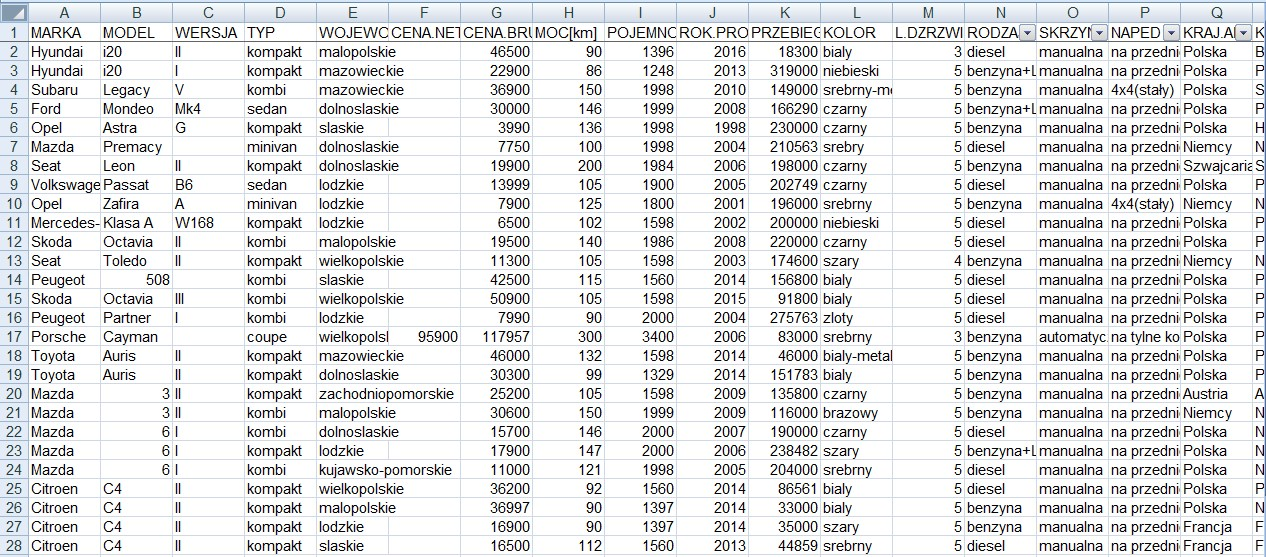
\includegraphics[width=1\textwidth]{zbior2}
%\caption{Podgląd stworzonego zbioru}
%\label{fig:obrazek1}
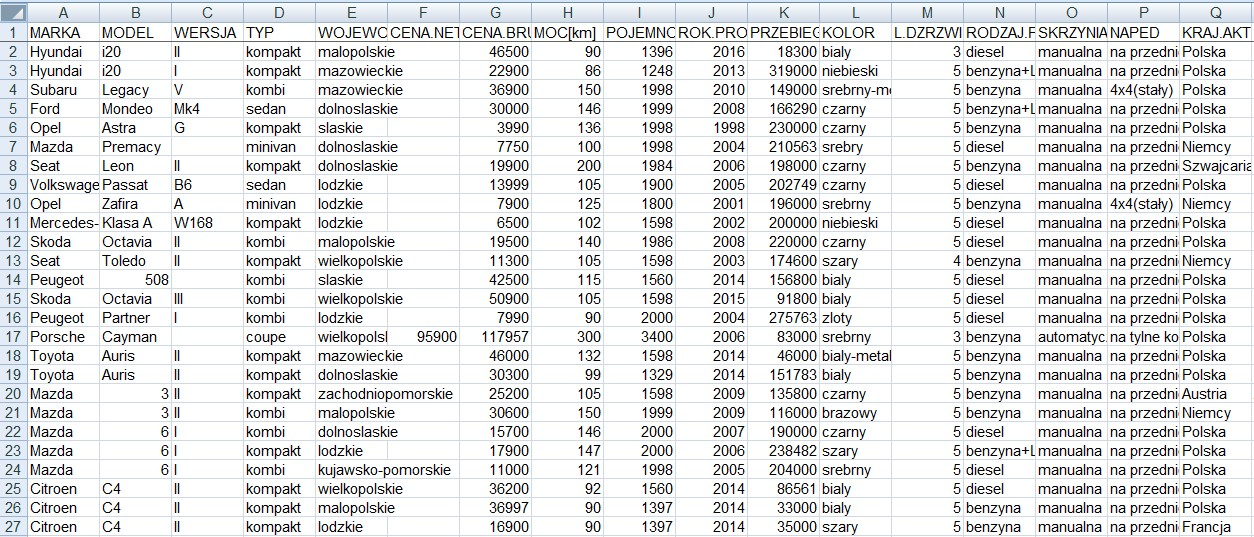
\includegraphics[width=1\textwidth]{img/zbior3.jpg}
\caption{Podgląd stworzonego zbioru}
\label{fig:obrazek1}
\end{figure}


\subsubsection{Użyte zmienne}


W stworzonym zbiorze danych znajduje się 29 atrybutów, opisujących 61 różnych rekordów, tj. obiektów reprezentowanych przez wiersze, którym przypisano pewne wartości atrybutów. Wśród zebranych danych można wyróżnić zarówno zmienne jakościowe, jak i ilościowe. 

Zmiennymi jakościowymi są atrybuty:
\begin{multicols}{3} 
\begin{itemize}
	\item marka,
	\item model,
	\item typ,
	\item wojewodztwo,
	\item kolor,
	\item rodzaj.paliwa,
	\item skrzynia.biegow,
	\item naped,
	\item kraj.aktualnej.rejestracji,%KRAJ.AKTUALNEJ.REJESTRACJI,
	\item kraj.pochodzenia,%KRAJ.POCHODZENIA,
	\item stan,
	\item ABS,
	\item uszkodzony,
	\item pierwszy.wlasciciel,%PIERWSZY.WLASCICIEL,
	\item kto.sprzedaje,%KTO.SPRZEDAJE,
	\item serwisowany,%SERWISOWANY,
	\item komputer.pokladowy,%KOMPUTER.POKLADOWY,
	\item ESP,
	\item klimatyzacja,%KLIMATYZACJA,
	\item bezwypadkowy,%BEZWYPADKOWY,
	\item status.pojazdu.sprowadzanego%STATUS.POJAZDU.SPROWADZONEGO.
\end{itemize}
\end{multicols}


Wśród zmiennych jakościowych można wyróżnić zmienne porządkowe, nominalne oraz binarne. W stworzonym zbiorze danych zmiennymi binarnymi są atrybuty: 
\begin{multicols}{3}
\begin{itemize}
	\item pierwszy.wlasciciel,%PIERWSZY.WLASCICIEL,
	\item ABS,
	\item serwisowany,%SERWISOWANY,
	\item komputer.pokladowy, %KOMPUTER.POKLADOWY
	\item ESP,
	\item bezwypadkowy,%BEZWYPADKOWY,
	\item uszkodzony.%USZKODZONY.
\end{itemize}
\end{multicols}

Pozostałe atrybuty są zmiennymi nominalnymi.

Zmiennymi ilościowymi są atrybuty:
\begin{multicols}{3}
\begin{itemize}
 \item cena.netto[pln],%CENA.[PLN].NETTO,
 \item cena.brutto[pln],% CENA.[PLN].BRUTTO
 \item moc,%MOC
 \item pojemnosc.skokowa[cm$^3$],% POJEMNOSC.SKOKOWA[cm3]
 \item rok.produkcji, %ROK.PRODUKCJI
 \item przebieg[km],%PRZEBIEG[km]
 \item l.drzwi. %L.DRZWI
\end{itemize}
\end{multicols}

Wśród zmiennych ilościowych można wyróżnić zmienne skokowe oraz dyskretne. W stworzonym zbiorze danych, zmiennymi skokowymi są: 
\begin{multicols}{3}
\begin{itemize}
	\item moc, %MOC
	\item pojemnosc.skokowa[cm$^3$], %POJEMNOSC.SKOKOWA[cm3]
	\item rok.produkcji, %ROK.PRODUKCJI
	\item przebieg, %PRZEBIEG,
	\item l.drzwi. %L.DRZWI

\end{itemize}
\end{multicols}
Z kolei atrybuty: cena.netto[pln], cena.brutto[pln] są zmiennymi ciągłymi. 
%czy zmienne porządkowe nie powinny być zaliczane do zmiennych ilościowych?
%l.drzwi powinna zostać zaliczona do zmiennych porządkowych 

\section{Użyte programy}
Zbiór danych został umieszczony w programie Excel, z kolei implementacje zostały opracowane przy wykorzystaniu programu R-Studio, który to jest niekomercyjnym programem mającym zastosowanie w statystyce i ekonometrii. 





\bibliographystyle{plain}
\bibliography{plik_z_bibliografia}





%% F1 F11 F1 F1
\end{document}
